% !TeX spellcheck = en_US
\documentclass[authoryear]{elsarticle}
\usepackage{amsmath}
\usepackage{amssymb}
\usepackage{float}
\usepackage{graphicx}
\usepackage{subcaption}
\usepackage{changepage}
\usepackage{url}
\usepackage{xfrac}
\usepackage{booktabs}
\usepackage{rotating}
\usepackage{geometry}
%\usepackage{authblk}
\usepackage{xcolor}
%\usepackage{colortbl}
\usepackage{multirow}
%\usepackage{blindtext}
%\usepackage{mathtools}
%\usepackage{titlesec}
%\setcounter{secnumdepth}{4}
%\usepackage{wasysym}
%\usepackage{cleveref}
%\DeclarePairedDelimiter{\ceil}{\lceil}{\rceil}
\usepackage{lineno}
\linenumbers
\usepackage{setspace}
\doublespacing
\usepackage[flushleft]{threeparttable}
\usepackage[colorlinks,citecolor=blue,urlcolor=blue]{hyperref} 
%\usepackage{titlesec}
%
%\setcounter{secnumdepth}{4}
%\titleformat{\paragraph}
%{\normalfont\normalsize\bfseries}{\theparagraph}{1em}{}
%\titlespacing*{\paragraph}
%{0pt}{3.25ex plus 1ex minus .2ex}{1.5ex plus .2ex}

%\usepackage{apacite}
\bibliographystyle{elsarticle-harv}

\makeatletter
\def\ps@pprintTitle{%
	\let\@oddhead\@empty
	\let\@evenhead\@empty
	\def\@oddfoot{\centerline{\thepage}}%
	\let\@evenfoot\@oddfoot}
\makeatother


\begin{document}
\begin{frontmatter}
	\title{
%		Anthropocentric uses of phosphorus: flows quantification and potential for recycling in Ontario
%	Mapping phosphorus flows in the economic sectors of Ontario and assessing recovery and recycling potential
%	Phosphorus in Ontario's economic sectors: flows mapping and recovery economic analysis
%	Phosphorus in Ontario's economic sectors: flows mapping and economic analysis of P recovery
Phosphorus flows mapping and economic analysis for its recovery in the province of Ontario, Canada
	}
	
	%% Group authors per affiliation:
	\author[ULaval]{Université Laval team\corref{mycorrespondingauthor}}
	\cortext[mycorrespondingauthor]{Corresponding author}
	\ead{edgar.martin-hernandez.1@ulaval.ca}
%	%\fntext[myfootnote]{Since 1880.}
	\author[McGill]{McGill University team}
	\author[Waterloo]{University of Waterloo team}
		
	\address[ULaval]{Université Laval}
	\address[McGill]{McGill University}
	\address[Waterloo]{University of Waterloo}
	
	\begin{abstract}
		The dual dimension of the anthropogenic use of phosphorus, i.e., its key role in the food production system and the negative environmental impacts associated with the phosphorus used in intensive agricultural techniques, has been stated by the United Nations Environment Assembly. In addition, phosphorus is a non-renewable material which reserves are concentrated in a few number of regions, making global supply chains vulnerable to regional events and conflicts. As a consequence, the recovery and recycling of phosphorus is not just a desirable but also a necessary approach to assure a sustainable, reliable, and sovereign food production system. In this work we map the phosphorus flows through the economic sectors of the Canadian province of Ontario, and phosphorus recovery and recycling opportunities are identified. These mainly belong to the agricultural sector, including manure (30.5 kt/year) and slaughterhouse waste (3.7 kt/year), although significant amounts of P are also found in food and organic waste, including municipal wastewater (6.4 kt/year). Different scenarios are studied to determine the amount of phosphorus that could be recovered within the province considering according with the technology readiness level of different phosphorus recovery processes, as well as the costs associated with phosphorus recovery {\color{red}Add some more numbers here}. Finally, we discuss the implications that would be derived from implementing active phosphorus recovery and recycling approaches regarding phosphorus supply and use in Ontario. 
	\end{abstract}
%	
%	\begin{keyword}
%		Quantifying P flows in Ontario's agricultural sector 
%	\end{keyword}
\end{frontmatter}

%\tableofcontents

\section{Introduction}
Phosphorus is an essential for production of food which has been intensively used for crop and livestock production since the development of synthetic fertilizers in the XIX and XX centuries \citep{Kausar19}. The combination of synthetic fertilizers with other modern intensive agricultural techniques have increased the productivity of agriculture and farming industries \citep{pingali2012green}.
However, the intensive use of fertilizers in agriculture has resulted in the over-application of phosphorus in many regions worldwide REF, while the run of intensive livestock production facilities, also known as concentrated animal feeding operations (CAFOs) \citep{animal_unit_definition}, result in important difficulties in the management of the large amounts of manure produced, which is often spread in lands in the vicinity of CAFOs, which also leads to the accumulation of phosphorus in soil. Soil acts as a phosphorus reservoir \citep{ehlert2003potential}, building-up a legacy P that can be used for future crops, but also can be transported to waterbodies by erosion and runoff leading to the eutrophication of aquatic ecosystems.

The dual dimension of the anthropogenic use of phosphorus, i.e., its key role in the food production system and the negative environmental impacts associated with the phosphorus used in intensive agricultural techniques, as it has been stated by the United Nations Environment Assembly in the resolution UNEP/EA.5/Res.2 \citep{UN_Phosphorus}. An additional factor to be considered for addressing the phosphorus challenge is the non-renewable nature of phosphorus, since the phosphorus consumed is not replenished by natural means at human time scale, and there is currently no known synthetic substitute for this material \citep{cordell2009story}. Since the global phosphorus reserves are concentrated in a few number of regions, the supply of phosphorus from a limited number of global supply chains lacks resiliency and it has been proven that it can be globally disrupted by regional events and conflicts, resulting geopolitical tensions \citep{FAO_UkraineWar}. As a consequence, the recovery and recycling of phosphorus is not just a desirable but also a necessary approach to assure a sustainable, reliable, and sovereign food production system. 

Although the main uses of phosphorus are in the agri-food sector, phosphorus is also involved in other industrial activities, including steel, chemical, and forestry industries. Henceforth, phosphorus is a key material for many aspects of human development. As a result, mapping the phosphorus flows involved in human activities to detect opportunities for recovery and recycling is essential for, in a second stage, assess amount of phosphorus that is viable to recover, the economical costs involved, and the enhancement in terms of resiliency of the regional food production system, savings from the reduction of phosphorus imports, and the mitigation of phosphorus pollution on the region implementing strategies for phosphorus recovery and recycling. The quantification of phosphorus flows has been addressed in previous works in the literature for certain sectors such as the agri-food sector \citep{boh2020nitrogen, zhou2021model, nesme2018global}. Additionally, studies on the global phosphorus flows have also been performed \citep{villalba2008global, chen2016half}, although these studies tend to have a low flow resolution since these are aggregated by major sectors. Additionally, the works quantifying phosphorus often include qualitative recommendations to improve the phosphorus use efficiency and recycling \citep{van2016phosphorus, senthilkumar2012conceptual}, but often they do not include quantitivae assessments on the amount of phopshorus which recovery is feasible along with the costs involved. Conversely, those works focused on estimating the recoverable phosphorus and the associated recovery cost target specific flows, lacking a holistic perspective of the phosphorus flows in the various human activities \citep{martin2021geospatial, sampat2018technologies}.

In this work, we intend to perform a holistic approach to phosphorus management,
%by mapping the phosphorus flows and identifying the opportunities for phosphorus
recovery, and recycling usingin the Canadian province of Ontario. In a first stage, we proceed to map the phosphorus flows involved in the economical sectors of Ontario, i.e., the agricultural, industrial, and urban sectors. This data is used in a second stage to identify the flows in which phosphorus recovery is feasible, estimating the amount of phosphorus that could be recovered within the province considering
%different scenarios regarding the technology readiness level of
different phosphorus recovery technologies with technology readiness levels equal or above 6, as well as the costs associated with phosphorus recovery. Finally, we discuss the implications that would be derived from implementing active phosphorus recovery and recycling approaches regarding phosphorus supply and use in Ontario.

\section{Methods}
%\subsection{Scope}
%We seek to quantify the phosphorus flows used in human activities, including the agricultural, urban, and industrial sectors. 

%The assessment is performed dividing the target sector in two subsectors, i.e., livestock and crop production, as shown in Fig. \ref{fig:Scope}. These subsectors are in turn sub-divided into specific activities, such as animal feeding, manure production, fertilizer application, etc.
%
%\begin{figure}[h!]
%	\centering
%	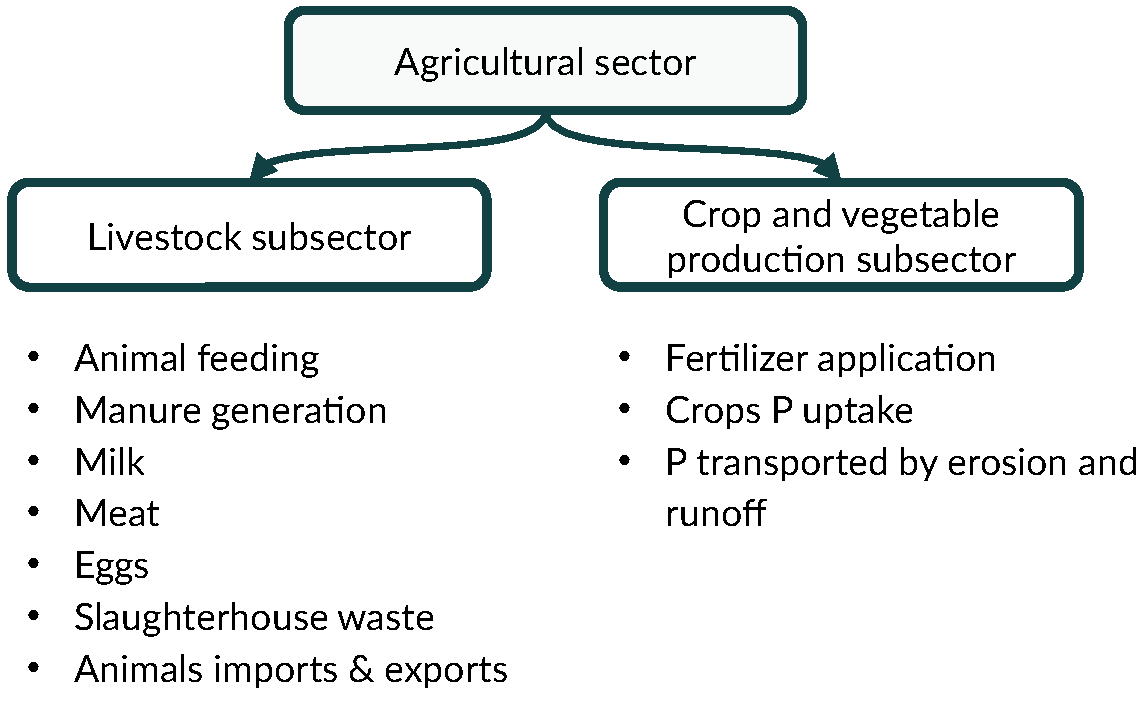
\includegraphics[width=0.7\linewidth, trim={0cm 0cm 0cm 0cm},clip]{gfx/scope.pdf} 
%	\caption{}
%	\label{fig:Scope}
%\end{figure}

\subsection{Spatial boundaries and resolution}
Phosphorus flows have been mapped within the Canadian province of Ontario, and thus the political borders of Ontario has been considered as the boundaries for the material flow analysis (MFA) performed \citep{brunner2016handbook}. In those cases where the data was availbale, the distribution of phosphorus flows within Ontario has also been studied at Census Division level \citep{CensusDivisionCD}. The database collecting the IDs of Ontario Census Divisions, their names, and geospatial information is taken from \citet{CensusDivisionOpendatasoft}.

{\color{red}Ask Melissa if we can reproduce the maps in the supplementary material}

{\color{red}ADD MAP WITH CENSUS DIVISIONS????}

\subsection{Temporal boundaries}
The study has being performed for year 2019 since the most of data required is available for this year. In addition, the temporal evolution of the largest phosphorus flows, i.e., agricultural and wastewater phosphorus flows, has been studied for a period of 13 years from 2007 to 2019.
%The study has being performed for years 2001-2021. However, for the years 2001-2006 and 2020-2021 there are some unavailable data, resulting in a partial loose resolution of the study. Therefore, the most complete information on agricultural P flows is reported for the years 2007-2019.

\subsection{Estimation of phosphorus flows}
The estimation of phosphorus flows within the Ontario's agricultural sectors is based on the methodology used in \citet{PFlows_Ontario}. It is based on the use open data sources, often from governmental institutions, complemented with information from scientific articles when needed. The particular procedure followed for each flow depends on the information publicly available. In the next sections we depict the main lines of the estimating procedure for each sector, {\color{red}while we refer the reader to \citet{PFlows_Ontario} for a more comprehensive description of the procedure followed for estimating each phosphorus flow.}

\subsubsection{Agricultural sector} \label{section:AgriSector}
Phosphorus flows in the agricultural sector are estimated based on production data of livestock and crop products, as well as data on fertilizer application.

For those production data were not available, a number of different
methods were used to estimate the P flow based on approaches established in the literature. For example, P inflows
associated with synthetic fertilizers could be directly estimated based on application data reported in the Fertilizer
Shipments Survey (FSS).37 Conversely, 
P flows associated with manure were determined indirectly by accounting for
the magnitude from which the flow of P could be derived. In this case, 

Phosphorus in livestock imports and exports is estimated from livestock trading data REF, multiplying the number of animals by the concentration of phosphorus in the different types of livestock REF,

Phosphorus in livestock feeding and manure
%meat and slaughterhouse waste
is estimated based on the number and type of animals reported for Ontario at Census Division level in the Census of Agriculture REF!, multiplied by the phosphorus feeding requirements REF, and concentration of phosphorus in manure REF.
%and carcasses REF respectively. 
The Census of Agriculture is published by Statistics Canada every five years (i.e., 2001, 2006, 2011, and 2016) for cattle52 REF, sheep53 REF, swine54 REF, poultry55 REF, and other livestock56 REF, with the exception of rabbits, where data is not available prior to 2009. The number of animals for the years in between census reporting have been estimated using a linear interpolation. We assumed that the number of animals reported is throughout the year (i.e., the animals culled are replaced by new ones). However, in the case of broilers and turkeys, the number of animals reported by the livestock census have been reduced by a factor of 0.68 (broilers) and 0.80 (turkeys), since these animals have life cycles of 43 and 80 days respectively, meaning barns are empty for 20 days between cycles. 305 REF

Phosphorus contained in meat and slaughterhouse waste is based on the number of animals slaughtered reported by both federally and provincially licensed meat plants.59, 60 REF multiplied by the concentration of phosphorus in carcasses REF.

Phosphorus flows associated with the production of milk and eggs is based on provincial production data, multiplying these products by their average phosphorus concentration 57, 58 REF.

Phosphorus in fertilizer applied to open fields in Ontario is estimated based on the amount of fertilizer products traded to Ontario’s agricultural markets containing P 100 REF. The distribution of phosphorus fertilizers among the Census Division of the province is based on the fraction of fertilized area of each census division, i.e., dividing the reported area of land fertilized for each census division by the total fertilized area of land in Ontario, removing the areas that correspond with greenhouse crops101, 102 103 REF. 
Regarding manure, we assume that all of the manure generated by livestock is applied in crop fields 50 REF.

The uptake of phosphorus by crops is determined based on the area used in each Census Division to grow each type of crops by census division104, 105, 106 and its yield107, 108 multiplied by the specific P content for each crop type.109, 110.  The phosphorus uptake by crops is divided according to whether it uptake in the grain, fruit or vegetable, or
straw and stover components of each type of crop. This is necessary to determine the amount of phosphorus that flows within food or feed (i.e.,grains, fruits and vegetables) while straw and stover remain in the field after harvesting as crop residues.

A fraction of the phosphorus applied to crop fields as manure of synthetic fertilizer is lost through erosion, runoff, and drainage. This transportation of phosphorus depends on a range of factor, including the amount of phosphorus applied; soil composition, texture, and slope; and precipitation, resulting in a complex and data-intensive process for estimating the phosphorus transported out of the crop fields. As an approximation, we have estimated the phosphorus losses by using export coefficients determined for crop fields in Ontario 112 REF 113 REF corrected to account for both surface and subsurface runoffs for synthetic fertilizers (1.267 kg/ha/year ), and liquid and solid manure (2.548 kg/ha/year and 1.717 kg/ha/year respectively) 113 REF \citep{PFlows_Ontario}.

A fraction of the P supplied to crop fields is not taken up by the plants and remains in soil, resulting in the accumulation of P over time as a result of synthetic fertilizer and manure over over sustained periods of time, often applying phosphorus in greater quantities than crops require to ensure satisfactory yields 132 REF. This buildup is often referred to as “legacy P”, and it is estimated as the balance between phosphorus inflows to crop fields (application of manure and synthetic fertilizers) and outflows (crop food and feed products, crop residues, and phosphorus losses).

Regarding greenhouse crops, the data available was limited, resulting in an estimation of phosphorus applied as synthetic fertilizers based on the sum of phosphorus uptake by greenhouse crops (i.e., tomatoes, peppers, and cucumbers)119 and the phosphorus releases from greenhouse irrigation systems (greenhouse nutrient feedwater systems (GNF) REF ONTARIO) systems. The phosphorus uptake by greenhouse crops is determined by multiplying the production of greenhouse crops 120 REF by the phosphorus content of each vegetable type 121, 122 REF. The phosphorus releases from the GNF systems was estimated based on the average concentration of phosphorus in GNF outlet streams of Ontario (33.6 mg/L) 123 REF and the total water discharges from GNF systems 124 REF, assuming that water discharges from GNF systems is equivalent to 25\% of the total water applied in greenhouses, which corresponding with the worst-case scenario of no water recirculation in the GNF system. The average water consumption in greenhouses in Ontario was assumed to be 1,000 L/m2/year 125 REF. We have also estimated the phosphorus releases from the seasonal workers live in households in the vicinity of the greenhouses that may use septic systems, considering that the seasonal labour force in Ontario greenhouses is estimated to be 6,699 workers 126 REF, and an average phosphorus load rate of f 0.0156 kg P/person/week from septic systems 128 REF.

{\color{red} REVISAR POR SIDNEY Food imports and exports (other than livestock)
are estimated scaling each type of food 
%available in Canada \citep{FoodAvailableCanada} 
traded in Canada \citep{TradeDataOnlineCanada}
with the population of Ontario \citep{PopulationCanada}.
%and then subtracting the amount of each type of food produced within Ontario.
The phosphorus contained in each type of imported and exported food is estimated multiplying the amount of ech type of traded food by its phosphorus content \citep{CanadianNutrientFile}.
}


\subsubsection{Industrial sector}
Phosphorus flows through imports, production, exports and waste for the steel, forestry, and food and beverage, industries of Ontario were mapped.
The steel industry is the first non-food sector in terms of phosphorus use. The main phosphorus inflows of steel manufacturing are associated with the use of iron ore, coal, and coke, while the main outflow of phosphorus is within slag, which remove most of the impurities from steel, including phosphorus. It must be noted that, although some minor amounts of phophosphorus can be desired in steel for making anti-corrosion surface coatings, it is largely considered an impurity in the steel manufacturing process. Phosphorus in these flows is estimated multiplyting their average phosphorus content (0.06\% P in iron ore, 0.05\% P for coal, 0.4\% P in slag, and 0.01\% in steel) 176 REF by the steel production capacity of the facilities located in Ontario \citep{CheminfoServices, AlgomaSteel, Stelco, PFlows_Ontario} and the imports and exports of these materials \citep{WorldIntegratedTradeSolution, InterprovincialImportsExports}.

Phosphorus flows in Ontario's forestry industry includes wood harvesting, wood products manufacturing, as well as the production of pulp and paper. The estimation of these phosphorus flows are the result of multiplying the production data of wood, wood products, pulp and paper, and their retrospectives imports, exports, and waste streams \citep{CanadianForestServiceStatistics, InterprovincialImportsExports}, by the average phosphorus content, which is assumed to be 0.01\% for wood 181 REF and 0.005\% for pulp and paper products REF.

Phosphorus in aquaculture are mainly due to supply of feed as part of fish feed the grow of trouts, part of which is uptake by fishes, while the rest of phosphorus is released into aquatic ecosystems since aquaculture effluents are directly discharged to the environment \citep{OntarioAquaculture}. The amount phosphorus uptakes by fishes
%supplied to aquaculture as fish feed is taken from, while the phosphorus uptakes by fishes are 
is calculated multiplying the fish production \citep{StatisticsCanadaAquaculture}, by their phosphorus content \citep{CanadianNutrientFile}, while the phosphorus content in the aquaculture waste effluents of Ontario is estimated to be 10 kg of phosphorus per ton of fish produced \citep{bureau2003chemical}. The sum of phosphorus uptakes by fishes and phosphorus in aquaculture waste effluents result in the phosphorus supplied to aquaculture as fish feed.

Regarding other industrial activities which could involve the use of phosphorus, the local production of phosphorus is assumed to be negligible since phosphorus is not mined or refined in Ontario, and the synthetic phosphorus fertilizer imports are accounted in the agricultural section. The general chemical facilities located in Ontario report 350 t/year of phosphorus as waste REF, in addition of imports and exports of chemical products REF. However, there exist a significant fraction of phosphorus used in the industrial sector that cannot be tracked due to the lack of data.

{\color{red}Ask sidney what to do with food industry, and pet feed. My approach is to merge all of them as it is currently in the figure, but confirm with her}

\subsubsection{Urban sector}
In this section we include the phosphorus inflows and outflows through wastewater treatment plants (WWTPs), septic systems, and food and organic waste management facilities (landfills, composting sites, and anaerobic digestion facilities).

{\color{red}Jorge do you mind if the purposes of the papaer we stick with just one method? I think it is better, otherwise it becomes lengthy and confusing}

Phosphorus flows through WWTPs is estimated combining data from the National Pollutant Release Inventory (NPRI) REF, a public database of releases, disposals and transfers of pollutants, including industrial facilities, and data from the Wastewater Systems Effluent Regulations (WSER) database REF. Since the NPRI only contains data of those facilities that meet certain regulatory requirements, the information of this database must be complemented with the data from the WSER database, which includes information of Canadian WWTPs at the federal, provincial, and municipal level. The estimations on phosphorus flows through WWTPs are valitaed using the Municipal Treated Wastewater Effluent (MTWE) database REF, which collects annual data on water quality data and effluent levels for WWTPs in Ontario. {\color{red}We note that this data set only provides information about phosphorus releases from municipal WWTPs, but it does not collect phosphorus disposals and transfers. REVISAR POR JORGE.} This methodology is shown in Figure \ref{fig:MethodWWTPs}

{\color{red}Ask Jorge if I can make a new Figure}

\begin{figure}[H]
	\centering
	%	\begin{subfigure}[t]{0.5\linewidth}
	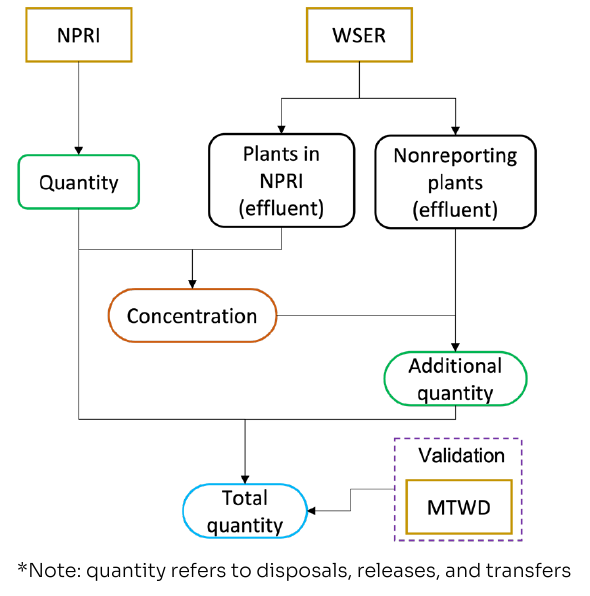
\includegraphics[width=0.5\linewidth, trim={0cm 0cm 0cm 0cm},clip]{Figures/TEmporary.png} 
	\caption{Methodology used for estimating phosphorus flows through wastewater treatment plants.}
	\label{fig:MethodWWTPs}
\end{figure}

However, there exist households that are not connected to any sewer systems. These households are equipped with septic systems to perform a rough treatment of the wastewater produced prior to its release into the environment, which typically consist into a septic tank that separates solid matter from the wastewater, and a drainfield where the effluent is discharged. The estimation of phosphorus releases from septic systems is based on the fraction of households equipped with these systems, estimated on 13\% \citep{CanadaSepticSystems}, which are inhabited by an average of 2.58 individuals \citep{CanadaPersonPerHouse}, and the average phosphorus load rate from septic systems, which is estimated on 0.81 kg of phosphor per person per year for the Lake Erie Basin in Ontario by \citet{oldfield2020estimation}.

Phophorus flows in the form of food and organic waste are based on applying food loss factors for the steps associated with food processing \citep{FoodLossesFAO}, considering the food production and import values estimated in Section \ref{section:AgriSector}.

\subsection{Phosphorus recovery techniques}
There exist different processes for phosphorus recovery from different sources at technologies readiness levels of 6 or above, i.e., at commercial or pilot plant stage. Since the flows from different processes have different properties, the techniques for phosphorus recovery vary, as well as their recovery efficiencies and products obtained. Table \ref{table:TechParam} shows a summary of the specifications of the phosphorus recovery technologies for different streams, as well as literature references with comprehensive descriptions of each system. We noted that the phosphorus recovery processes currently available exceed the systems included in this work, nonetheless the processes considered are a selection of the main techniques for phosphorus recovery, although different processes may have been developed through the fundamentals of the same technique, e.g., struvite precipitation. These table is based on different processes at different development level, from commercial to pilot plant stages.
%A collection of phosphorus recovery technologies for different streams can be found in the Table ??? of the Supplementary Material. 
%Different scenarios are studied considered the technology readiness level (TRL) of the processes in order to determine the phosphorus that could be immediately recovered using commercial technologies (Scenario 1), the phosphorus that could be recovered in a near future by using technologies above pilot plant development stage (Scenario 2), and finally  prospective assessment of phosphorus recovery systems that at early research stages (Scenario 3). 

Phosphorus recovery costs include operating and annualized capital costs. Capital costs are annualized through the application of an annual capital charge ratio $\left( ACCR\right)$ as defined by \citet{towler2013chemical}, assuming a typical interest rate of 5\% and a plant lifetime of 20 years. Dynamic phosphorus recovery costs in function of the processing capacity have been considered in order to capture the economies of scale for those technologies for which sufficient data are available.


\begin{table}[h]
%\begin{sidewaystable}[ph!]
	\centering
	\caption{ADD $F$ denotes the phosphorus recovered as $\sfrac{\text{kg P}_{\text{recovered}}}{\text{year}}$, while $\lceil x \rceil$ represent the ceiling function applied to $x$. The definition of annual capital charge ratio $\left( ACCR\right)$ can be found in the Supplementary Material, Section ??.} \label{table:TechParam}
	\resizebox{1.08\columnwidth}{!}{
				\begin{threeparttable}
		\begin{tabular}{@{}cccccccccc@{}}
			\toprule
			Sector                        & Inflow                                                                                                                                                  & Pretreatment                                                                     & \begin{tabular}[c]{@{}c@{}}Pretreatment cost\\ (EUR/kg P\textsubscript{recovered})\end{tabular} & Technology                                                                               & Type                                                                              & \begin{tabular}[c]{@{}c@{}}P recovery potential\\ (\% related to inflow)\end{tabular} & P recovery cost (EUR/kg P recovered) & TRL                                   & Ref tech \\ \midrule
			\multirow{27}{*}{Agriculture} & \multirow{10}{*}{\begin{tabular}[c]{@{}c@{}}Cattle and swine manure, \\ liquid phase\\ (30\% of total manure P)\end{tabular}}                               & \begin{tabular}[c]{@{}c@{}}Solid-liquid separation\\ (screw press)\end{tabular} &        See [1]                                & Multiform                                                                                & Struvite                                                                          & 60                                                                                    & $25.7 + 1.10 \cdot 10^6 \cdot \lceil 1.19 \cdot 10^{-4} \cdot F \rceil \cdot ACCR \cdot \frac{1}{F}$                                 & 9                                                            & [1]    \\
			&                                                                                                                                                         & \begin{tabular}[c]{@{}c@{}}Solid-liquid separation\\ (screw press)\end{tabular} &  See [1]                                      & Crystalactor                                                                             & \begin{tabular}[c]{@{}c@{}}Struvite/\\ Calcium phosphate\end{tabular}                                           & 60                                                                                    & $3.53 + \left( 2.30 \cdot 10^6 + 0.71 \cdot \lceil 3.32 \cdot 10^{-5} \cdot F \rceil\right)\lceil 3.32 \cdot 10^{-5} \cdot F \rceil \cdot ACCR \cdot \frac{1}{F} $                                  & 9                                                            &[1]          \\
			&                                                                                                                                                         & \begin{tabular}[c]{@{}c@{}}Solid-liquid separation\\ (screw press)\end{tabular} &   See [1]                                     & Ostara Pearl 500                                                                             & Struvite                                                                          & 60                                                                                    &  $12.57 + 2.30 \cdot 10^6 \cdot \lceil 7.02 \cdot 10^{-5} \cdot F \rceil \cdot ACCR \cdot \frac{1}{F}$                                & 9                                                            & [1]         \\
			& & \begin{tabular}[c]{@{}c@{}}Solid-liquid separation\\ (screw press)\end{tabular} &    See [1]                                    & Ostara Pearl 2K                                                                             & Struvite                                                                          & 60                                                                                    & $12.57 + 3.10 \cdot 10^6 \cdot \lceil 1.83 \cdot 10^{-5} \cdot F \rceil \cdot ACCR \cdot \frac{1}{F}$                                 & 9                                                            &  [1]        \\
			& & \begin{tabular}[c]{@{}c@{}}Solid-liquid separation\\ (screw press)\end{tabular} &     See [1]                                   & Ostara Pearl 10K                                                                             & Struvite                                                                          & 60                                                                                    &  $12.57 + 10.00 \cdot 10^6 \cdot \lceil 3.65 \cdot 10^{-6} \cdot F \rceil \cdot ACCR \cdot \frac{1}{F}$                                  & 9                                                            &   [1]       \\
			&                                                                                                                                                         & \begin{tabular}[c]{@{}c@{}}Solid-liquid separation\\ (screw press)\end{tabular} &             See [1]                           & Nuresys                                                                                  & Struvite                                                                          & 60                                                                                    & $10.37 + 1.38 \cdot 10^6 \cdot \lceil 2.24 \cdot 10^{-5} \cdot F \rceil \cdot ACCR \cdot \frac{1}{F}$                                  & 9                                                            & [1]         \\
%			&                                                                                                                                                         & \begin{tabular}[c]{@{}c@{}}Solid-liquid separation\\ ( screw press)\end{tabular} &                                        & P-RoC                                                                                    & Calcium phosphate                                                                 & 60                                                                                    & 36.8                                 & 6                                                            &          \\
			&                                                                                                                                                         & \begin{tabular}[c]{@{}c@{}}Solid-liquid separation\\ (screw press)\end{tabular} &   See [1]                                     & MAPHEX                                                                                   & Solid                                                                             & 90                                                                                    & $184.67 + 0.30 \cdot 10^6 \cdot \lceil 2.47 \cdot 10^{-4} \cdot F \rceil \cdot ACCR \cdot \frac{1}{F}$                                  & 6                                                            &     [1]     \\ \cmidrule(l){2-10}
			& \multirow{7}{*}{\begin{tabular}[c]{@{}c@{}}Cattle and swine manure, \\ solid phase\\ (70\% of total manure P)\end{tabular}}                                & Incineration                                                                     & 8.9                                    & EcoPhos                                                                                  & Phosphoric acid                                                                   & 82                                                                                    & 4.5                                  & 6                                                            & [2,3,4]    \\ 
			&                                                                                                                                                         & Incineration                                                                     & 8.9                                    & AshDec depollution                                                                       & Calcium phosphate                                                                 & 86                                                                                    & 1.8                                  & 6                                                            &   [2,3,4] \\
			&                                                                                                                                                         & Incineration                                                                     & 8.9                                    & AshDec Rhenania                                                                          & Calcium phosphate                                                                 & 86                                                                                    & 1.9                                  & 6                                                            &   [2,3,4] \\
			&                                                                                                                                                         & Incineration                                                                     & 8.9                                    & PASCH                                                                                    & Calcium phosphate                                                                 & 79                                                                                    & 4.7                                  & 6                                                            &  [2,3,4]  \\
			&                                                                                                                                                         & Incineration                                                                     & 8.9                                    & LEACHPHOS                                                                                & Calcium phosphate                                                                 & 78                                                                                    & 5.1                                  & 9                                                            &  [2,3,4]  \\
			&                                                                                                                                                         & Incineration                                                                     & 8.9                                    & RecoPhos                                                                                 & Mineral                                                                           & 87                                                                                    & 2.5                                  & 9                                                            & [2,3,4]   \\
			&                                                                                                                                                         & Incineration                                                                     & 8.9                                    & Thermophos                                                                               & P4                                                                                & 81                                                                                    & 2.7                                  & 9                                                            &  [2,3,4]  \\ \cmidrule(l){2-10}
			& Poultry litter                                                                                                                                          & -                                                                               & -                                     & Quick wash                                                                               & Solid precipitate                                                                 & 70                                                                                    & 4.4                                  & 3   &    [5]      \\ \cmidrule(l){2-10}
			& \multirow{4}{*}{\begin{tabular}[c]{@{}c@{}}Slaughterhouse waste, \\ liquid phase\\ (14\% of total slaughterhouse P)\end{tabular}}                    & -                                                                               & -                                     & Multiform                                                                                & Struvite                                                                          & 84                                                                                    & $22.6 + 1.10 \cdot 10^6 \cdot \lceil 1.05 \cdot 10^{-4} \cdot F \rceil \cdot ACCR \cdot \frac{1}{F}$                                 & 9                                                           &  [6]  \\
			&                                                                                                                                                         & -                                                                               & -                                     & Ostara Pearl 500                                                                             & Struvite                                                                          & 58                                                                                    & $15.60 + 2.30 \cdot 10^6 \cdot \lceil 8.70 \cdot 10^{-5} \cdot F \rceil \cdot ACCR \cdot \frac{1}{F}$                                 & 9                                                            &     [6]     \\
			&                                                                                                                                                         & -                                                                               & -                                     & Ostara Pearl 2K                                                                             & Struvite                                                                          & 58                                                                                    & $15.60 + 3.10 \cdot 10^6 \cdot \lceil 2.26 \cdot 10^{-5} \cdot F \rceil \cdot ACCR \cdot \frac{1}{F}$                                 & 9                                                            &    [6]      \\
			&                                                                                                                                                         & -                                                                               & -                                     & Ostara Pearl 10K                                                                             & Struvite                                                                          & 58                                                                                    & $15.60 + 10.00 \cdot 10^6 \cdot \lceil 4.53 \cdot 10^{-6} \cdot F \rceil \cdot ACCR \cdot \frac{1}{F}$                                 & 9                                                            &    [6]      \\ \cmidrule(l){2-10}
			& \multirow{7}{*}{\begin{tabular}[c]{@{}c@{}}Slaughterhouse waste, \\ solid phase\\ (86\% of total slaughterhouse P)\end{tabular}}                     & Incineration                                                                     & 14.6                                   & EcoPhos                                                                                  & Phosphoric acid                                                                   & 82                                                                                    & 4.5                                  & 6                                                            &   [2,3,7] \\
			&                                                                                                                                                         & Incineration                                                                     & 14.6                                   & AshDec depollution                                                                       & Calcium phosphate                                                                 & 86                                                                                    & 1.8                                  & 6                                                            &  [2,3,7]  \\
			&                                                                                                                                                         & Incineration                                                                     & 14.6                                   & AshDec Rhenania                                                                          & Calcium phosphate                                                                 & 86                                                                                    & 1.9                                  & 6                                                            &   [2,3,7] \\
			&                                                                                                                                                         & Incineration                                                                     & 14.6                                   & PASCH                                                                                    & Calcium phosphate                                                                 & 79                                                                                    & 4.7                                  & 6                                                            &   [2,3,7] \\
			&                                                                                                                                                         & Incineration                                                                     & 14.6                                   & LEACHPHOS                                                                                & Calcium phosphate                                                                 & 78                                                                                    & 5.1                                  & 9                                                            &  [2,3,7]  \\
			&                                                                                                                                                         & Incineration                                                                     & 14.6                                   & RecoPhos                                                                                 & Mineral                                                                           & 87                                                                                    & 2.5                                  & 9                                                            &  [2,3,7]  \\
			&                                                                                                                                                         & Incineration                                                                     & 14.6                                   & Thermophos                                                                               & P4                                                                                & 81                                                                                    & 2.7                                  & 9                                                            &  [2,3,7]  \\ \cmidrule(l){1-10}
			\multirow{36}{*}{\begin{tabular}[c]{@{}c@{}}Urban \& \\ industrial\end{tabular}}       & \multirow{6}{*}{\begin{tabular}[c]{@{}c@{}}WWTPs\\ (liquid phase)\end{tabular}}                                                                         & -                                                                               & -                                     & Crystalactor                                                                             & \begin{tabular}[c]{@{}c@{}}Struvite/\\ Calcium phosphate\end{tabular}                                                         & 38                                                                                    & $305,920 \cdot \left( \frac{F}{24,966} \right)^{0.59} \cdot \frac{1}{F}$                                 & 9                                                            &     [3]     \\
			&                                                                                                                                                         & -                                                                               & -                                     & Ostara Pearl                                                                             & Struvite                                                                          & 20                                                                                    & $130,856 \cdot \left( \frac{F}{13,140} \right)^{0.36} \cdot \frac{1}{F}$                                  & 9                                                            &   [3]       \\
			&                                                                                                                                                         & -                                                                               & -                                     & P-RoC                                                                                    & Calcium phosphate                                                                 & 27                                                                                    & $75,970 \cdot \left( \frac{F}{17,739} \right)^{0.78} \cdot \frac{1}{F}$                                  & 6                                                            &    [3]      \\
			&                                                                                                                                                         & -                                                                               & -                                     & REM-NUT                                                                                  & Struvite                                                                          & 47                                                                                    & $977,933 \cdot \left( \frac{F}{30,879} \right)^{0.94} \cdot \frac{1}{F}$                                 & 6                                                            &   [3]       \\
			&                                                                                                                                                         & -                                                                               & -                                     & AirPrex                                                                                  & Struvite                                                                          & 15                                                                                    & $74,195 \cdot \left( \frac{F}{9,855} \right)^{0.38} \cdot \frac{1}{F}$                                  & 9                                                            &     [3]     \\
			&                                                                                                                                                         & -                                                                               & -                                     & PRISA                                                                                    & Struvite                                                                          & 18                                                                                    & $186,923 \cdot \left( \frac{F}{11,826} \right)^{0.43} \cdot \frac{1}{F}$                                  & 6                                                            &     [3]     \\ \cmidrule(l){2-10}
			& \multirow{5}{*}{\begin{tabular}[c]{@{}c@{}}WWTPs \\ (sewage sludge,\\ 60-90\% of P)\end{tabular}}                                                       & -                                                                               & -                                     & Stuttgart process                                                                        & Struvite                                                                          & 40                                                                                    & $581,730 \cdot \left( \frac{F}{26,280} \right)^{0.89} \cdot \frac{1}{F}$                                 & 9                                                            &   [3]       \\
			&                                                                                                                                                         & -                                                                               & -                                     & Gifhorn process                                                                          & Struvite                                                                          & 40                                                                                    & $400,384 \cdot \left( \frac{F}{26,280} \right)^{0.82} \cdot \frac{1}{F}$                                    & 9                                                            &   [3]       \\
			&                                                                                                                                                         & -                                                                               & -                                     & PHOXNAN                                                                                  & Struvite                                                                          & 51                                                                                    & $891,667 \cdot \left( \frac{F}{33,507} \right)^{0.84} \cdot \frac{1}{F}$                                 & 6                                                            &    [3]      \\
			&                                                                                                                                                         & -                                                                               & -                                     & Aqua Reci                                                                                & Calcium phosphate                                                                 & 61                                                                                    & $939,605 \cdot \left( \frac{F}{40,077} \right)^{0.82} \cdot \frac{1}{F}$                                 & 6                                                            &    [3]      \\
			&                                                                                                                                                         & -                                                                               & -                                     & MEPHREC                                                                                  & P rich slag                                                                       & 68                                                                                    & $1,154,473 \cdot \left( \frac{F}{44,676} \right)^{0.61} \cdot \frac{1}{F}$                                 & 6                                                            &    [3]      \\ \cmidrule(l){2-10}
			& \multirow{7}{*}{\begin{tabular}[c]{@{}c@{}}WWTPs \\ (sewage sludge ash SSA,\\ 60-90\% of P)\end{tabular}}                                               & Incineration                                                                     & 8                                      & EcoPhos                                                                                  & Phosphoric acid                                                                   & 82                                                                                    & 4.5                                  & 6                                                            &    [3]      \\
			&                                                                                                                                                         & Incineration                                                                     & 8                                      & AshDec depollution                                                                       & Calcium phosphate                                                                 & 86                                                                                    & 1.8                                  & 6                                                            &    [3]      \\
			&                                                                                                                                                         & Incineration                                                                     & 8                                      & AshDec Rhenania                                                                          & Calcium phosphate                                                                 & 86                                                                                    & 1.9                                  & 6                                                            &     [3]     \\
			&                                                                                                                                                         & Incineration                                                                     & 8                                      & PASCH                                                                                    & Calcium phosphate                                                                 & 79                                                                                    & 4.7                                  & 6                                                            &     [3]     \\
			&                                                                                                                                                         & Incineration                                                                     & 8                                      & LEACHPHOS                                                                                & Calcium phosphate                                                                 & 78                                                                                    & 5.1                                  & 9                                                            &     [3]     \\
			&                                                                                                                                                         & Incineration                                                                     & 8                                      & RecoPhos                                                                                 & Mineral                                                                           & 87                                                                                    & 2.5                                  & 9                                                            &      [3]    \\
			&                                                                                                                                                         & Incineration                                                                     & 8                                      & Thermophos                                                                               & P4                                                                                & 81                                                                                    & 2.7                                  & 9                                                            &    [3]      \\ \cmidrule(l){2-10}
			& \multirow{8}{*}{\begin{tabular}[c]{@{}c@{}}Organic municipal\\ \& food waste\end{tabular}} & -                                                                               & -                                     & \begin{tabular}[c]{@{}c@{}}Chemical extraction and\\ Struvite precipitation\end{tabular} & Struvite                                                                          & 94                                                                                    & 24.8                                 & 3  &  [8]        \\                                              & & Incineration                                                                     & 6.43                                      & EcoPhos                                                                                  & Phosphoric acid                                                                   & 82                                                                                    & 4.5                                  & 6                                                            &   [3,9,10]       \\
			&                                                                                                                                                         & Incineration                                                                     & 6.43                                      & AshDec depollution                                                                       & Calcium phosphate                                                                 & 86                                                                                    & 1.8                                  & 6                                                            &    [3,9,10]      \\
			&                                                                                                                                                         & Incineration                                                                     & 6.43                                      & AshDec Rhenania                                                                          & Calcium phosphate                                                                 & 86                                                                                    & 1.9                                  & 6                                                            &    [3,9,10]      \\
			&                                                                                                                                                         & Incineration                                                                     & 6.43                                      & PASCH                                                                                    & Calcium phosphate                                                                 & 79                                                                                    & 4.7                                  & 6                                                            &     [3,9,10]     \\
			&                                                                                                                                                         & Incineration                                                                     & 6.43                                      & LEACHPHOS                                                                                & Calcium phosphate                                                                 & 78                                                                                    & 5.1                                  & 9                                                            &      [3,9,10]    \\
			&                                                                                                                                                         & Incineration                                                                     & 6.43                                      & RecoPhos                                                                                 & Mineral                                                                           & 87                                                                                    & 2.5                                  & 9                                                            &     [3,9,10]     \\
			&                                                                                                                                                         & Incineration                                                                     & 6.43                                      & Thermophos                                                                               & P4                                                                                & 81                                                                                    & 2.7                                  & 9                                                            &     [3,9,10]     \\ 
%			\cmidrule(l){1-10}
%			\multirow{2}{*}{Industrial}   & \multirow{2}{*}{Steel production}                                                                                                                       & -                                                                               & -                                     & Reductive melting                                                                        & \begin{tabular}[c]{@{}c@{}}I have doubts if this P\\ can be recycled\end{tabular} & ?                                                                                     &                                      & 5                                                             &          \\
%			&                                                                                                                                                         & -                                                                               & -                                     & \begin{tabular}[c]{@{}c@{}}Selective leaching–chemical\\ Precipitation\end{tabular}      & \begin{tabular}[c]{@{}c@{}}I have doubts if this P\\ can be recycled\end{tabular} & ?                                                                                     &                                      & 4                                                             &          
%			\\
			\bottomrule
%			\cmidrule(l){3-10} 
		\end{tabular}
					\begin{tablenotes}
						\footnotesize
						\item 1: \citet{martin2021geospatial}
						\item 2: \citet{jupp2021phosphorus}
						\item 3: \citet{egle_phosphorus_2016}
						\item 4: \citet{schoumans2010phosphorus}
						\item 5: \citet{szogi2008phosphorus}
						\item 6: \citet{Pearl2Kcost2}
						\item 7: \citet{zagklis2020assessing}
						\item 8: \citet{fernandez2022phosphorus}
						\item 9: \citet{ohtake2019phosphorus}
						\item 10: \citet{sharma2021life}
					\end{tablenotes}
			\end{threeparttable}
	}
%\end{sidewaystable}
\end{table}



\section{Results and discussion}
\subsection{Phosphorus flows in Ontario}
\emph{\color{red}Showing an overview of the P flows in the province. The use of figures summarizing all the flows of the province in the shape of Sankey or network flow figures could be so great}

\begin{figure}[H]
	\centering
	%	\begin{subfigure}[t]{0.5\linewidth}
	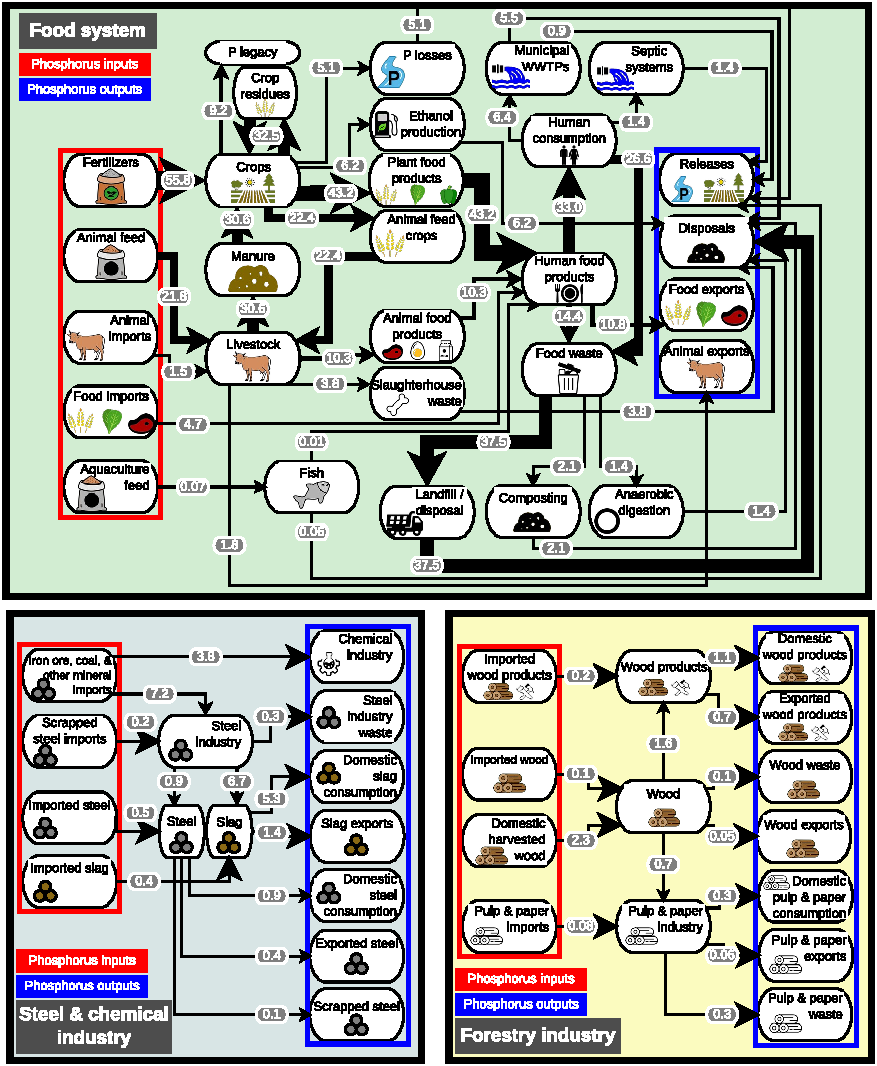
\includegraphics[width=1\linewidth, trim={0cm 0cm 0cm 0cm},clip]{Figures/Diagram2-3.pdf} 
	\caption{Phosphorus flows in the province of Ontario (kt/year). The streams within red rectangles denote phosphorus inflows into the province, while those streams within blue rectangles denote phosphorus outflows out of the province.}
	\label{fig:FigFlowsSummary}
\end{figure}

Figure \ref{fig:FigFlowsSummary} summarizes the phosphorus flows in the province of Ontario. It can be observed that the flow of of phosphorus through the anthropogenic activities are divided into 3 independent networks, i.e., the flow of phosphorus involved the production and processing of food (including the treatment of wastewater), the flow of phosphorus used in the steel and chemical industries, and the phosphorus involved in the forestry industry.

The production of animal food products exhibits a lower phosphorus use efficiency than the production of plant base products, similarly to the use effciciency of other resources such as water CITE HERE, CALCULAR ENTRA VS SALE!

\subsubsection{Agricultural sector}

\subsubsection{Industrial sector}

\subsubsection{Urban sector}

\subsection{Potential of phosphorus recovery in Ontario}
Assessment of different scenarios of P recovery in Ontario, P imports that would be saved, reduction of P dependency of the province, etc (all implications related with mass-balances)

\subsubsection{Scenario 1: phosphorus recoverable with current technologies}

\paragraph{\textbf{Agricultural sector}}
Phosphorus can be recovered from different flows within the agricultural sector, including the production of manure. Phosphorus recovery from cattle and swine manure is performed through struvite precipitation REF REF, existing different processes for struvite production at commercial stage, as described in Section ?REF?. Phosphorus recovery from poulty litter is based on acid extraction and further precipitation \citep{szogi2008phosphorus}. Since this technology shows a lower development level, their use has been considered in Scenario 2, see Section ??.  \citet{martin2021geospatial} determined that the implementation of struvite production processes at livestock facilities is mainly driven by the scale of the CAFO, and thus they can be divided by into three clusters regarding the type of phosphorus recovery processes implemented, i.e., facilities with capacity for between 300 and 2,000 animal units, for between 2,000 and 5,000 animals units, and facilities large than 5,000 animal units. An animal unit (AU) is defined as an animal equivalent of 1,000 pounds (453.6 kg) live weight \citep{animal_unit_definition}. The most suitable phosphorus recovery for process for the facilities of each one of these clusters was determined by \citet{martin2021geospatial}, resulting in that  Multiform-type processes are the most suitable struvite produciton system for the cluster including the small-size CAFOs cluster (300-2,000 AUs), NuReSys-type systems are suitable for medium-size CAFOs (2,00-5,000 AUs), while that the suitable struvite system for large-scale CAFOs is Crystalactor-type processes. The investment and operating cost of these systems is collected in Table ?REF?.

The number of cattle animals is reported by the Census of Agriculture at Census Division level REF, but no available data on CAFOs size is available for the province of Ontario. Since this information is essential to determine the suitable phopshorus recovery process to be considered, and in turn the phosphorus recovery cost, the distribution of CAFOs sizes has been approximated to the cattle and swine CAFOs size distribution of other regions in the vicinity of the Great Lakes area, namely Ohio, Pennsylvania, Indiana, Michigan, and Wisconsin. The distribution of CAFOs size in each one of these regions has been approximated through a truncated normal distribution, since the possible size of livestock facilities is bounded between 300 animal units for being considered as an intensive livestock production facility REF, and 10,000 animal units in order to remove extra-large CAFOs that are outliers in the size distribution, avoiding excessive long tails distorting the distributions.
For cattle CAFOs, it has been found that two scenarios can be identified, a first scenario (Scenario 1) where the average size of CAFOs is larger, around 2,400 animal units based on the parameters of the states of Ohio, Wisconsin, and Michigan, and a second scenario (Scenario 2) based on the states of Pennsylvania and Indiana where the average size of CAFOs is smaller, lower than 1,500 animal units. Two CAFOs size distributions are proposed for Ontario based on each one of these scenarios, estimating the parameters of Eq. REF as the average parameters of the distributions in each scenario, as shown in \ref{fig:CAFOsSize_Scenarios}. 
For swine CAFOs, the size distribution patterns are similar for all the states studied, with the exception of the Wisconsin, which has been discarded due to the little number of swine facilities installed in this state. A truncated normal distribution with mean equal to 741 AUs and standard deviation equal to 456 AUs is assumed to stimate the distribution of swine CAFOs in Ontario, as shown in \ref{fig:CAFOsSize_Scenarios}.
The distribution parameters for both cattle and swine CAFOs size are shown in Table \ref{table:CAFOsSizeScenarios}.
The number of CAFOs in each cluster is determined through the Monte Carlo method, with the constrain that the sum of animal units of all CAFOs must not exceed the total number of animal units of Ontario, which for cattle is equal to 1,376,984 animal units for year 2019, which result in the release of 15,923 kt of manure per year and 13.27 kt of phosphorus per year, and for swine represent 506,768 animal units, 5,779 kt of manure per year, and 8.57 kt of phosphorus per year REF. The number of CAFOs belonging to each cluster are shown in Table \ref{table:CAFOsSizeScenarios}. Further details on the estimation of CAFOs size distribution can be found in the Supplementary Information, Section ??.

\begin{figure}[H]
	\centering
	\begin{subfigure}[t]{0.49\textwidth}
		\centering
		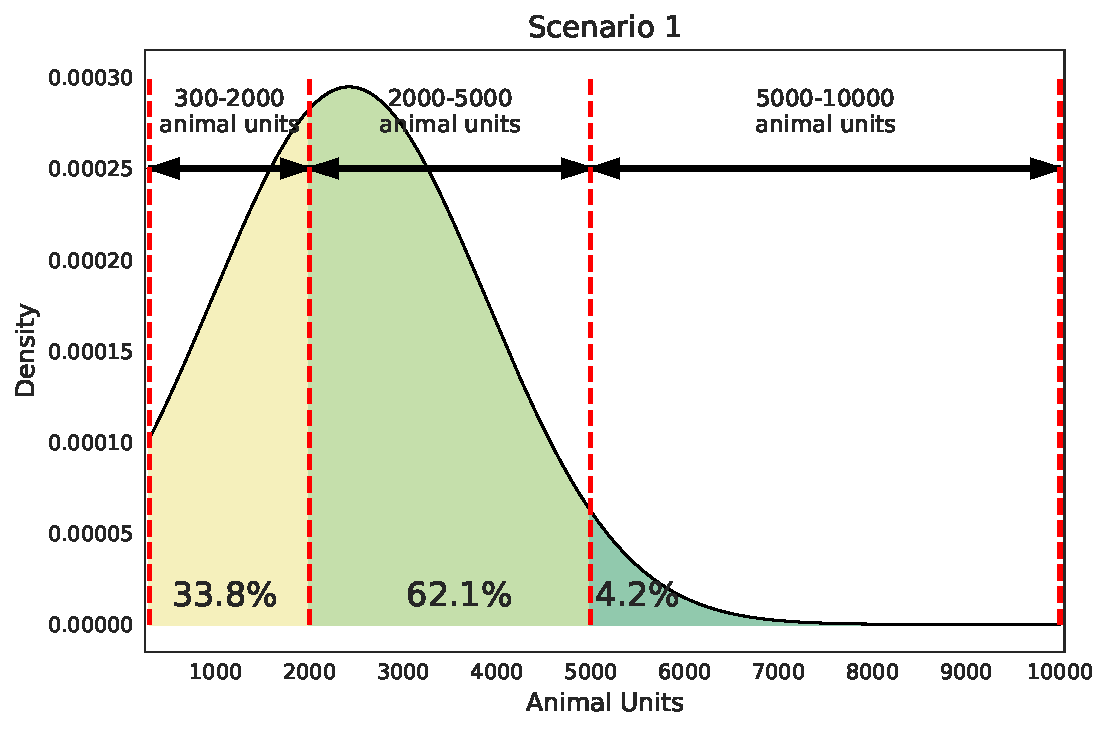
\includegraphics[width=\linewidth, trim={0.2cm 0.2cm 0.7cm 0.7cm},clip]{Figures/Scenario1_CAFOs_Size_Distribution.pdf} 
		\caption{Cattle (scenario 1)}
		\label{fig:CAFOsSize_Scenario1}
	\end{subfigure}
	\begin{subfigure}[t]{0.49\textwidth}
		\centering
		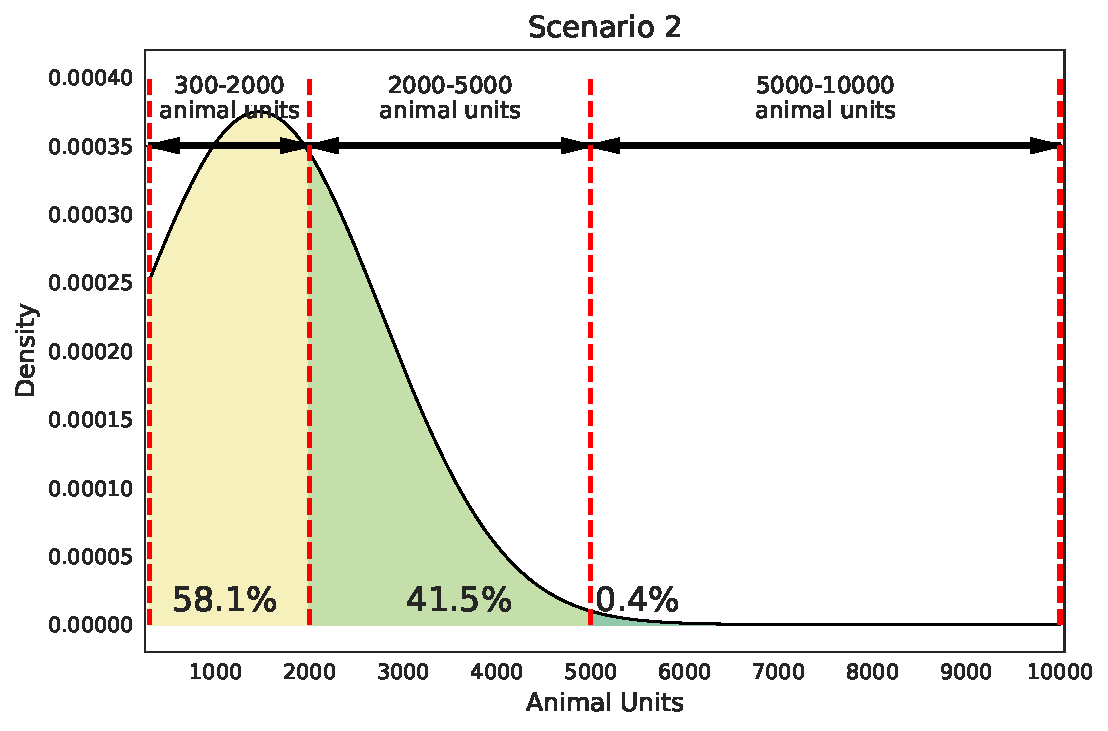
\includegraphics[width=\linewidth, trim={0.2cm 0.2cm 0.7cm 0.7cm},clip]{Figures/Scenario2_CAFOs_Size_Distribution.pdf}
		\caption{Cattle (scenario 2)}
		\label{fig:CAFOsSize_Scenario2}
	\end{subfigure}

\vspace{0.5cm}

	\begin{subfigure}[t]{0.49\textwidth}
		\centering
		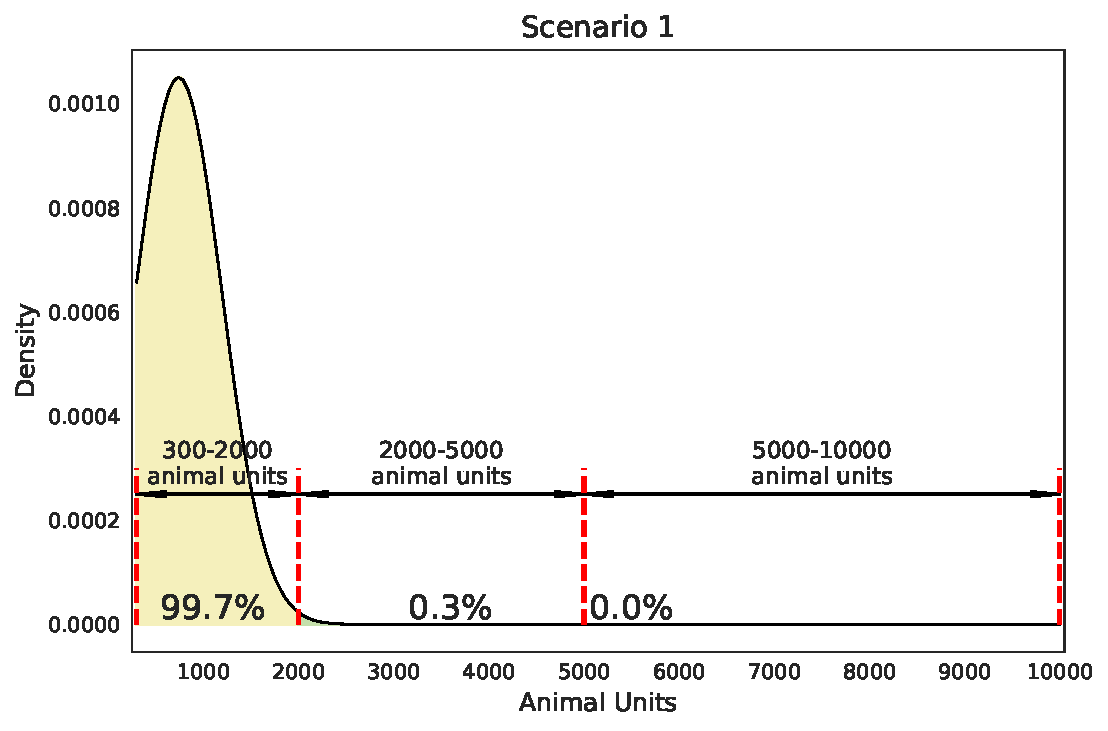
\includegraphics[width=\linewidth, trim={0.2cm 0.2cm 0.7cm 0.7cm},clip]{Figures/Scenario1_SwineCAFOs_Size_Distribution.pdf}
		\caption{Swine}
		\label{fig:CAFOsSize_Scenario2}
	\end{subfigure}
	
	\caption{Proposed distribution of CAFOs size in the province of Ontario based on the size distribution of cattle and swine facilities in other regions in the vicinity of the Great Lakes area. Cattle scenario 1 is based on the pattern shown by the US states of Ohio, Wisconsin, and Michigan, which shows an average CAFO size around 2,4000 animal units, while cattle scenario 2 is based on the pattern shown by the US states of Pennsylvania and Indiana, with an average CAFO size around 1,3000 animal units.}
	\label{fig:CAFOsSize_Scenarios}
\end{figure}

\begin{table}[h]
	\centering
	\caption{Truncated normal distribution parameters and number of CAFOs in each cluster for the scenarios studied regarding cattle and swine CAFOs size distribution.} \label{table:CAFOsSizeScenarios}
	\resizebox{0.6\columnwidth}{!}{
		%		\begin{threeparttable}
		\begin{tabular}{@{}cccc@{}}
			\toprule
			Parameter & Cattle (scenario 1) & Cattle (scenario 2) & Swine \\ \midrule
			mean                                                                              & 2,423.40   & 1,463.94 & 741.42    \\
			std                                                                               & 1,459.70   & 1,308.91 & 455.71   \\
			a                                                                                 & 300        & 300  & 300    \\
			b                                                                                 & 10,000        & 10,000 & 10,000     \\
			\begin{tabular}[c]{@{}c@{}}Number of CAFOs\\ (300-2,000 AU)\end{tabular}           & 177        & 386 & 575        \\
			\begin{tabular}[c]{@{}c@{}}Number of CAFOs\\ (2,000-5,000 AU)\end{tabular}          & 324        & 319   & 2     \\
			\begin{tabular}[c]{@{}c@{}}Number of CAFOs\\ (\textgreater{}5,000 AU)\end{tabular} & 22         & 3    & 0      \\
			Total AUs & 13,76,984 & 13,76,984 & 506,768 \\ \bottomrule
		\end{tabular}
		%			\begin{tablenotes}
		%				\footnotesize
		%				\item 1: \citet{MilkOntario}
		%			\end{tablenotes}
		%	\end{threeparttable}
	}
\end{table}

\paragraph{\textbf{Industrial sector}}
Slaughterhouse waste is a waste flow from food industry which can be targeted for phosphorus recovery. Phosphorus can be recovered from the wastewater produced in slaughterhouses through struvite precipitation \citep{Pearl2Kcost2}, and from the solid residues from animal carcasses \citep{jupp2021phosphorus}. Phosphorus technologies suitable for phosphorus recovery from these sources are collected in Table \ref{table:TechParam}. Data on individual capacities for the slaughterhouses in Ontario is not available for estimating the effects of the economies of scale, and therefore average slaughterhouse capacities of 104,017, 802,186, and $14.4 \cdot 10^6$ cattle, hog, and poultry heads slaughtered per year respectively are assumed \citep{SlaughterhouseDistribution, SlaughterhousePoultryAverageSize}, resulting in 7, 6, and 17 catlle, hog, and poultry slaughtering facilities with associated phosphorus flows of 317.4, 103.5, and 53.2 metric tonnes/$\left(\text{facility} \cdot \text{year}\right) $ respectively. Phosphorus flows from sheep and rabbit slaughtered are considered negligible. The number of slaughtered animals can be found in Table ?? of Supplementary Material.

\paragraph{\textbf{Urban sector}}
Municipal wastewater contains significant amounts of phosphorus that can be recovered. It must be noted that phosphorus outflows from WWTPs are divided into phosphporus contained in the treated water and phosphorus contained in sludge. Phosphorus contained in water can be recovered through the formation of precipitates such as struvite, while phosphorus contained in sludge can be recovered either through the direct processing of sludge producing precipitates, of from sludge ashes after an incineraiton stage, obtaining different products such as phosphoric acid or calcium phosphare, as shown in Table \ref{table:TechParam}. The distribution of phosphorus between treated water and sludge considered is 14.1\% - 85.9\% respectively \citep{PFlows_Ontario}, based on the data reproted by NPRI and WSER databases REFs, which in alignment with the distribution values reported by \citep{egle_phosphorus_2016}.

\subsection{Economic implications of phosphorus recovery in Ontario}
Economic costs or saving derived from the recovery of P in the province and all implications related with economy

\subsection{Implications on food sovereignty of phosphorus recovery in Ontario}
Implications on food production self-sufficiency derived from the (partial) recycling of P. Discussion on the improvement of the food production system resiliency against disruptions of the global supply supply chains  (e.g., current context derived from the COVID-19 pandemia and the war in Ukraine)

\subsection{Gaps of knowledge}

\section{Conclusions}

\section{Acknowledgments}
{\color{red}Pollution Probe}

{\color{red}ECCC}

%\section{Livestock sector}
%Phosphorus flows in the livestock sector can be defined taking the animal as reference, i,e., P inputs in the form of animal feeding, and P outputs, which include manure, milk, eggs, meat, and carcasses, as shown in Fig. \ref{fig:LivestockPFlows}.
%
%\begin{figure}[h!]
%	\centering
%	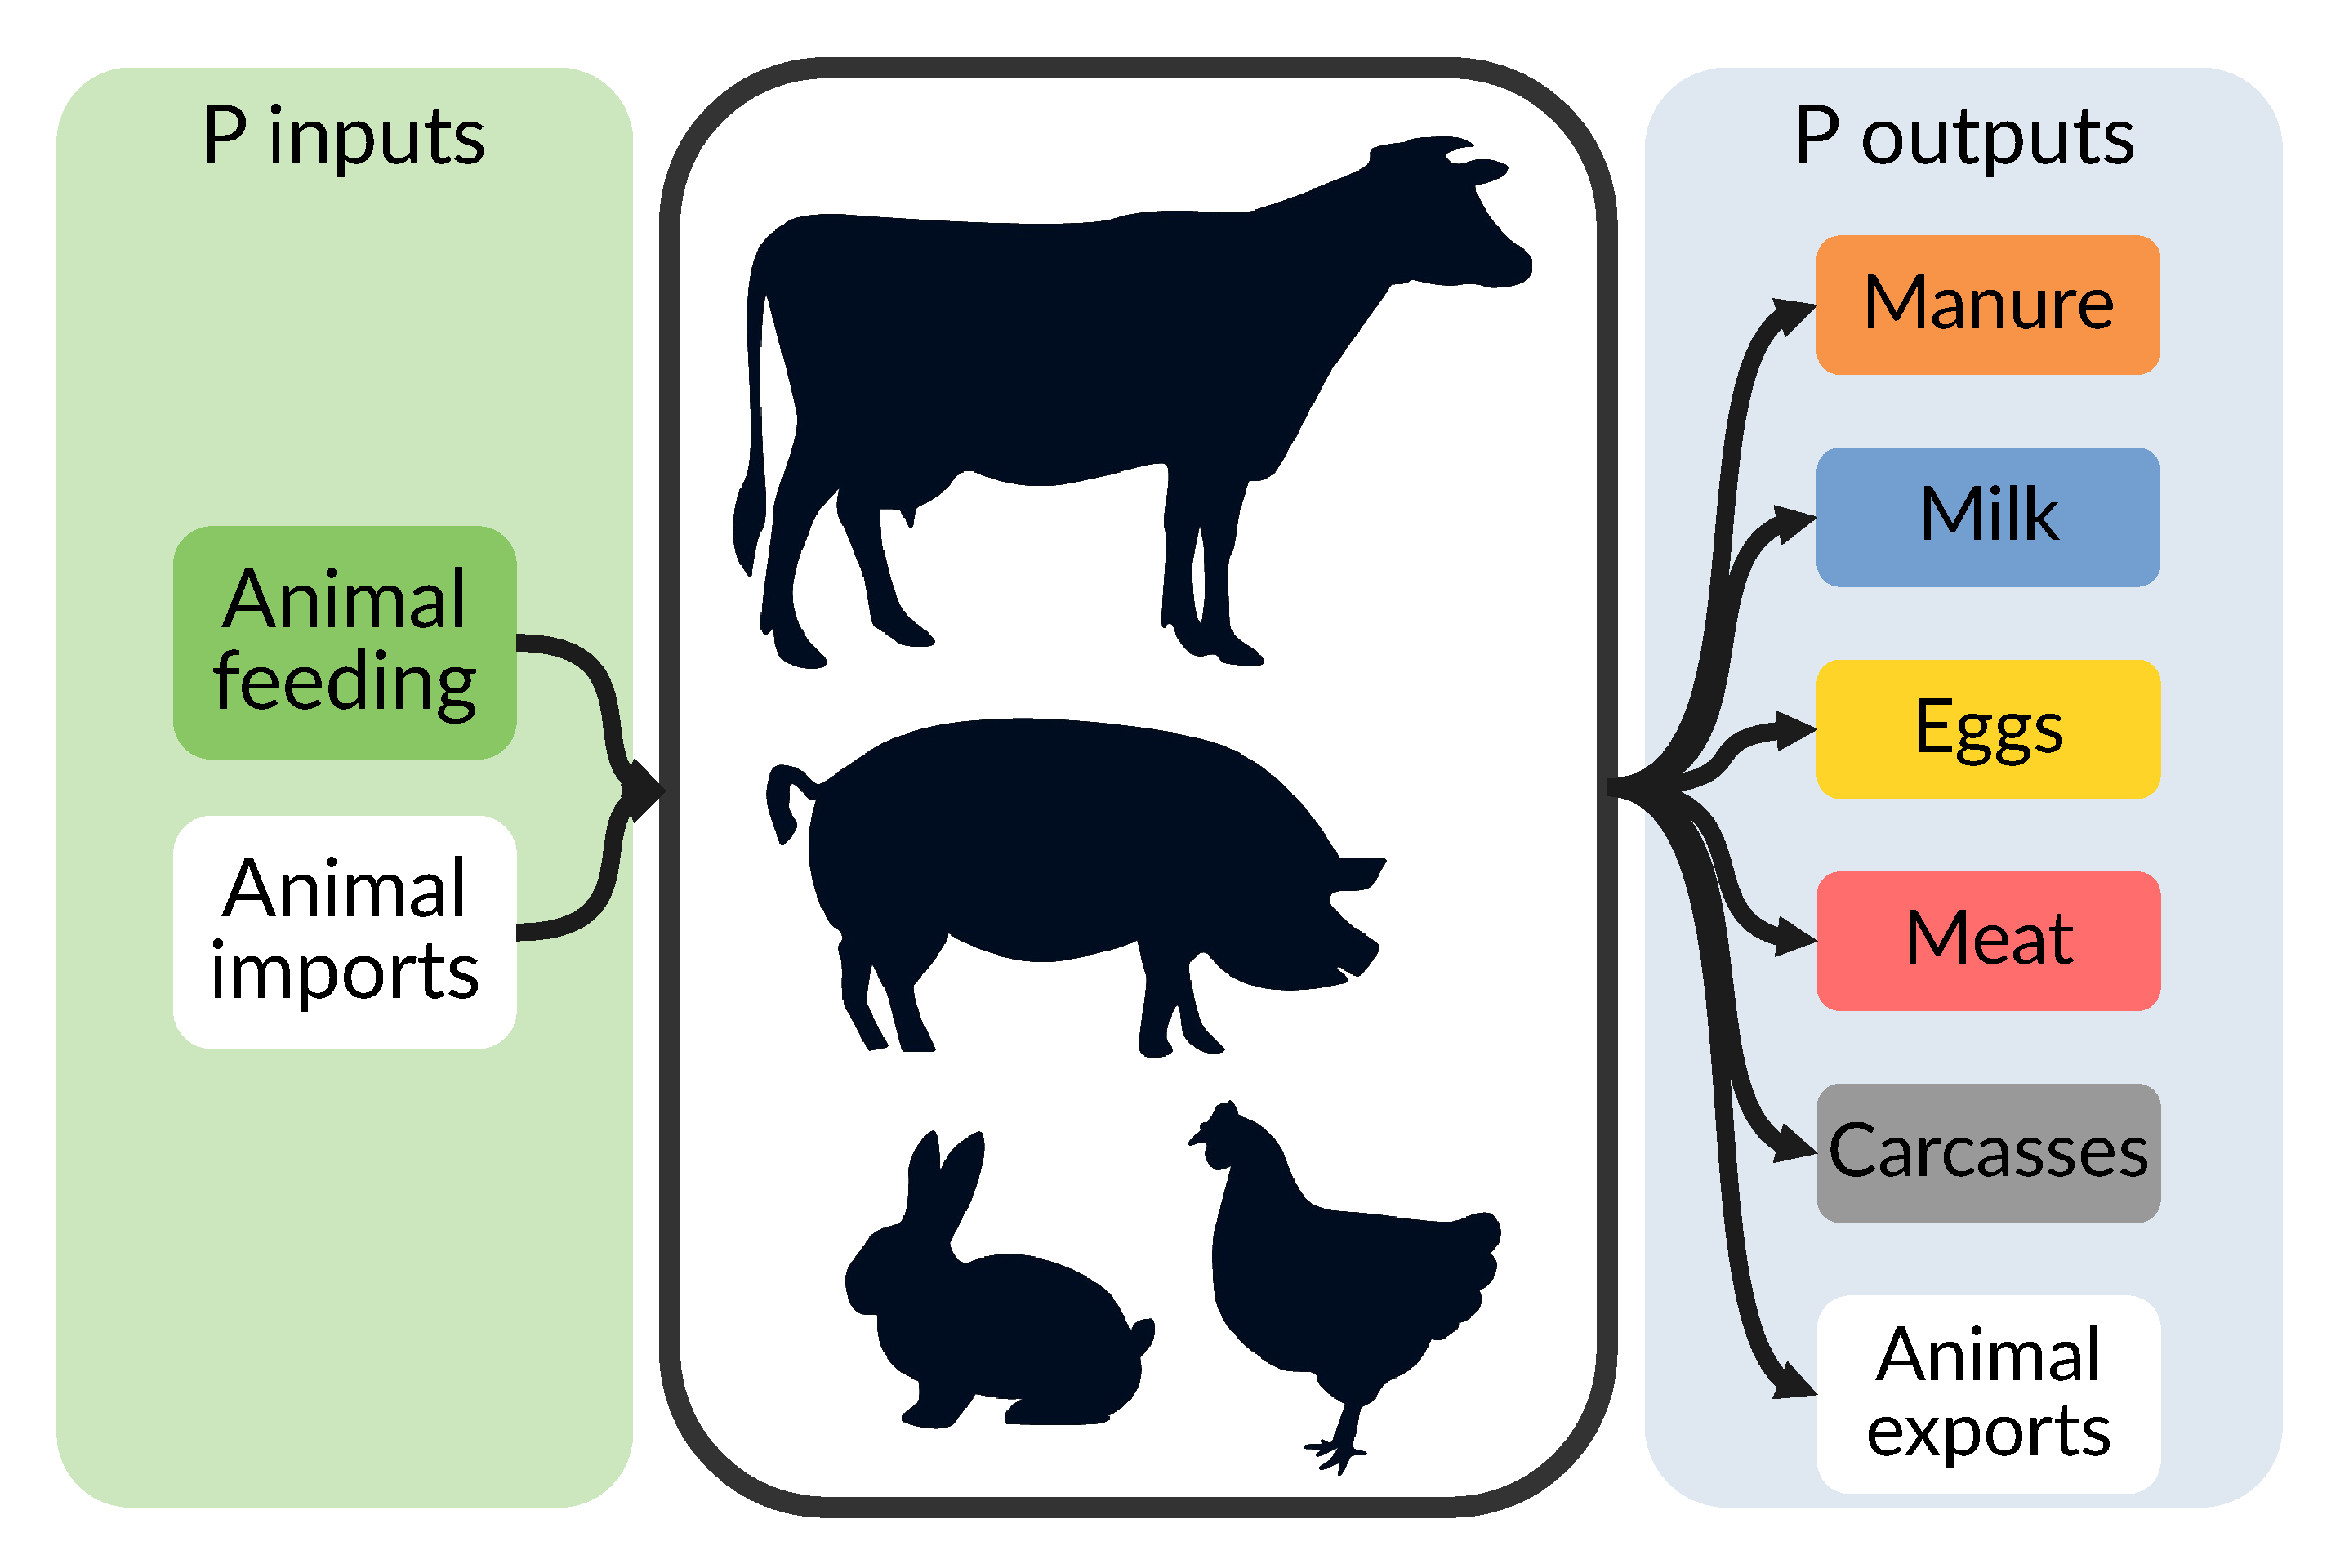
\includegraphics[width=0.6\linewidth, trim={0cm 0cm 0cm 0cm},clip]{gfx/LivestockPFlows.pdf} 
%	\caption{}
%	\label{fig:LivestockPFlows}
%\end{figure}
%
%\subsection{Livestock census} \label{section:LivestockCensus}
%Livestock census is retrieved from the Census of Agriculture performed by Statistics Canada -- Statistique Canada every five years, i.e, 2001, 2006, 2011, and 2016, for cattle \citep{LivestockCensusCattle}, sheep \citep{LivestockCensusSheep}, swine \citep{LivestockCensusPig}, poultry \citep{LivestockCensusPoultry}, and other livestock \citep{LivestockCensusOtherLivestock}. The inventory of rabbits is not available prior 2009.
%
%Livestock census is reported using Dissemination Geography Unique Identifiers (DGUIDs). These identifiers are built based on 4 items combined in a unique DGUID identifier: vintage (4 digits representing the year of data collection), the type of geographic areas covered by the dataset (1 character code, A or S denoting administrative or statistical areas respectively), the schema (4 digits item denoting the kind of division considered. 0003 denotes Census Division), and the Geographic Unique Identifier (GEOUID) (variable alphanumeric code assigned to each individual geographical division), which in this case corresponds with the Census Divisions of Ontario identifier (a 4 digits code starting by `35') \citep{DGUID}. The GEOUID is extracted from the DGUID reported by the census using Pandas \citep{mckinney-proc-scipy-2010} to retrieve the number of animals of each type in each Census Division.
%
%\textcolor{red}{The inventory of animals for the years between two consecutive Census of Agriculture has been estimated through a linear interpolation between the data of consecutive census.}
%
%\subsection{Correction by animal production cycles} \label{section:CorrectionProductionCycles}
%The livestock census provides a snapshot of the number of animals in the region studied. We assumed that the number of animals reported is maintained constant along the year (i.e., the animals culled are replaces by new ones). However, in the case of broiler and turkey the number of animals reported by the livestock census have been reduced by a factor of 0.68 and 0.80 respectively, since these animals have life cycles of 43 and 80 days respectively, maintaining the barns empty for 20 days between cycles, as reported by \citet{yang2007development}.
%
%\subsection{P flows in manure}
%\subsubsection{Manure generation}
%Each type of animal has been in turn classified in different groups attending its different life stages as listed below. Moreover, a number of assumptions have been considered for the animal under evaluation to estimate the P released in the form of manure, which are listed below. The manure produced by elk, deer, and wild boar farming could not be accounted due to the lack of data regarding manure generation.
%
%\begin{itemize}
%	\item \textbf{Cattle:} Dairy cows, beef cows, beef calves, and dairy heifers are differentiated based on the data on manure generation and composition available.
%	\begin{itemize}
%		\item Bulls and steers have been considered comparable to beef cows.
%		\item Calves have been considered beef calves.
%		\item Due to the lack of data for beef heifers and dairy heifers are merged as dairy heifers.
%	\end{itemize}
%	
%	\item \textbf{Swine:} Mature and immature animals are differentiated based on the data on manure generation and composition available.
%	\begin{itemize}
%		\item Grower and finishing pigs, nursing pigs, and weaner pigs have been considered as immature pigs.
%		\item Sows and gilts for breeding, and boars have been considered as mature pigs.
%	\end{itemize}
%	
%	\item \textbf{Sheep:} Sheep and lambs are differentiated based on the data on manure generation and composition available. 
%	\begin{itemize}
%		\item Ewes and rams have been considered as sheep.
%	\end{itemize}
%	
%	\item \textbf{Poultry:} Chicken broilers and pullets, laying hens, and turkeys are differentiated based on the data on manure generation and composition available. 
%	\begin{itemize}
%		\item Broilers, roasters, cornish. and other poultry have been considered comparable to chicken broilers.
%		\item Layer and broiler breeders (pullets and hens), and pullets under 19 weeks, intended for laying table eggs, are considered chicken pullets.
%		\item Laying hens, 19 weeks and over, that produce table eggs are considered chicken layers.
%	\end{itemize}
%
%		\item \textbf{Horses:} Based on the data on manure generation and composition available, all horses are considered as a single animal type. 
%	\begin{itemize}
%		\item Horses and ponies are all considered horses.
%	\end{itemize}
%	\item \textbf{Goats:} Based on the data on manure generation and composition available, all goats are considered as a single animal type. 
%	\item \textbf{Rabbit:} Based on the data on manure generation and composition available, all rabbits are considered as a single animal type. 
%	\item \textbf{Mink:} Based on the data on manure generation and composition available, all minks are considered as a single animal type. 
%	\item \textbf{Bison:} Based on the data on manure generation and composition available, all bison are considered as a single animal type. 
%	\item \textbf{Llamas and alpacas:} Based on the data on manure generation and composition available, llamas and alpacas could be evaluated separately. However, the data reported by the livestock census aggregate these type of animals \citep{LivestockCensusOtherLivestock}.
%	\begin{itemize}
%		\item The average values for manure generation and composition of llamas and alpacas have been considered.
%	\end{itemize}
%\end{itemize}
%
%
%Manure production in each Census Division is estimated for each type of animal under consideration combining the number of animals $\left(N_{animals} \right) $ reported by the livestock census and the manure production rate of each type of animal $\left(m \right) $, as shown in Eq. \ref{eq:ManureProd}.
%%reported by the U.S. Department of Agriculture \citep{USDAHandbook, Kellog2010}.
%
%\begin{align}
%	& Manure \left( \frac{\text{kg}}{\text{day}} \right)  = N_{animals_{i}} \left(\text{animals} \right) \cdot AU_{eq_{i}} \left( \frac{\text{AU}}{\text{animals}} \right) \cdot m_{i} \left( \frac{\text{kg}}{\text{day} \cdot \text{AU}}\right) \label{eq:ManureProd}  \\
%	& \forall \ i \ \in \big\{\text{Beef Cow, Dairy Cow, Beef Calf, Dairy Heifer, Swine Mature, Swine Inmature,} \nonumber \\
%	& \text{Sheep, Lamb, Broiler, Pullet, Chicke Layer, Turkey, Horse, Goat, Rabbit, Mink,} \nonumber \\
%	& \text{Bison,Llamas/Alpacas}\big\} \nonumber 
%\end{align}
%
%\subsubsection{P releases}
%The amount of P contained in manure is calculated based on the composition reported for each type of manure, as shown in Eq. \ref{eq:PProd} \citep{USDAHandbook, Kellog2010, vallentine1990grazing, pagliari2012investigation, barnett1994phosphorus, BrownCompositions, NetherlandsCompositions, NSCompositions,
%%abdoli2014feasibility, 
%NERCCompositions}. These values are collected in Table \ref{table:waste}.
%
%\begin{align}
%	& P_{manure} \left( \frac{\text{kg}}{\text{day}} \right)  = Manure \left( \frac{\text{kg}}{\text{day}} \right) \cdot P_{total} \left(\%\text{wt}\right) \label{eq:PProd}
%\end{align}
%
%\begin{table}[H]
%	\centering
%	\caption{Manure generation rates and composition for different types of animals.}
%	\label{table:waste}
%	\resizebox{\columnwidth}{!}{
%	\begin{tabular}{@{}cccccccc@{}}
%		\toprule
%		Livestock type   & Water & Organic matter & N\textsubscript{total} & P\textsubscript{total} & K\textsubscript{total} & Manure & AU\textsubscript{eq} \\
%		 &(\%)&(\%)&(\%)&(\%)&(\%)&(kg/day/AU)& (AU/animals) \\ \midrule
%		Dairy cow        & 87         & 10.98               & 0.59              & 0.08              & 0.20              & 37.88              & 0.74       \\
%		Dairy heifer     & 83         & 13.04               & 0.48              & 0.09              & 0.21              & 29.95              & 0.94       \\
%		Dairy calf       & 83         & 9.28                & 0.51              & 0.06              & 0.13              & 29.95              & 4.00       \\
%		Beef cow         & 88         & 10.58               & 0.34              & 0.08              & 0.24              & 28.58              & 1.00       \\
%		Beef calf        & 88         & 10.00               & 0.58              & 0.10              & 0.38              & 28.14              & 4.00       \\
%		Swine mature     & 90         & 9.15                & 0.76              & 0.22              & 0.47              & 15.19              & 2.67       \\
%		Swine inmature   & 90         & 8.31                & 0.83              & 0.14              & 0.37              & 36.51              & 9.09       \\
%		Chicken layers   & 75         & 19.30               & 1.93              & 0.58              & 0.68              & 28.46              & 250.00     \\
%		Chicken pullets  & 75         & 19.30               & 1.93              & 0.58              & 0.68              & 20.68              & 455.00     \\
%		Chicken broilers & 75         & 19.09               & 1.09              & 0.32              & 0.62              & 37.21              & 455.00     \\
%		Turkey mature    & 74         & 20.42               & 1.50              & 0.42              & 0.65              & 22.67              & 50.00      \\
%		Turkey inmature  & 74         & 20.42               & 1.50              & 0.42              & 0.65              & 20.33              & 67.00      \\
%		Sheep            & 75         & 20.75               & 1.13              & 0.18              & 0.75              & 18.16              & 5.00       \\
%		Lamb             & 75         & 20.75               & 1.13              & 0.18              & 0.75              & 18.16              & 7.14       \\ 
%		Mink             & 54         & 45.80               & 3.28              & 1.82              & 0.79              & 42.74              & 150.00     \\
%		Horses           & 85         & 11.92               & 0.60              & 0.13              & 0.37              & 23.38              & 0.91       \\
%		Rabbits          & 54         & 46.00               & 1.22              & 0.87              & 0.57              & 51.64              & 50.00      \\
%		Goat             & 68.8       & 31.20               & 1.06              & 0.37              & 1.03              & 20.94              & 5.88       \\
%		Llamas/alpacas   & 69         & 31.00               & 0.71              & 0.38              & 0.24              & 12.49              & 3.50       \\
%		Bison            & 78.9       & 21.10               & 0.40              & 0.07              & 0.07              & 44.88              & 0.91       \\
%		\bottomrule
%	\end{tabular}
%	}
%\end{table}
%
%\subsection{P flows in agricultural products}
%\subsubsection{P flows in milk}
%The production of milk in Ontario has been retrieved at county level from the statistical data reported by \citet{MilkOntario}. These data is available for the years 2007 to 2020. However, not all counties directly align with Census Division, and the data of some counties have been merged or broken down in order to obtain the data for the corresponding Census Divisions. In those cases where county data have been broken down into several Census Divisions, this procedure has been performed proportionally to the number of dairy cows in the targeted Census Division over the total number of dairy cows in the original county. The number of cows at Census Division level is obtained from \citet{LivestockCensusCattle}, see section \ref{section:LivestockCensus} for more details.
%
%\begin{table}[h]
%	\centering
%	\caption{Distribution and characteristics studied CAFOs, and phosphorus recovery processes selected. Only selected technologies are included in the table.} \label{table:techs_intalled}
%	\resizebox{0.8\columnwidth}{!}{
%	\begin{threeparttable}
%		\begin{tabular}{@{}ccc@{}}
%%			\centering
%			\toprule
%			\begin{tabular}[c]{@{}c@{}}Counties reported\\ in [1]\end{tabular} & \begin{tabular}[c]{@{}c@{}}Equivalent\\ Census Divisions\end{tabular}                                                                                        &\begin{tabular}[c]{@{}c@{}}Operation\\ performed\end{tabular}  \\ \midrule
%			Essex and Kent                                                           & Essex; Chatham-Kent                                                                                                                                          & Break down          \\
%			Haldimand; Norfolk                                                       & Haldimand-Norfolk                                                                                                                                            & Merge               \\
%			Hamilton-Wentworth                                                       & Hamilton                                                                                                                                                     & Rename              \\
%			Dundas; Glengarry; Stormont                                              & Stormont, Dundas and Glengarry                                                                                                                               & Merge               \\
%			Grenville; Leeds                                                         & Leeds and Grenville                                                                                                                                          & Merge               \\
%			Ottawa-Carleton                                                          & Ottawa                                                                                                                                                       & Rename              \\
%			Prescott; Russell                                                        & Prescott and Russell                                                                                                                                         & Merge               \\
%			Others                                                                   & \begin{tabular}[c]{@{}c@{}}Sudbury; Greater Sudbury / Grand Sudbury;\\ Parry Sound; Nipissing; Manitoulin;\\ Toronto; Haliburton; Kenora; Muskoka\end{tabular} & Break down          \\ \bottomrule
%	\end{tabular}
%	\begin{tablenotes}
%				\footnotesize
%				\item 1: \citet{MilkOntario}
%	\end{tablenotes}
%	\end{threeparttable}}
%%	}
%\end{table}
%
%The P content of milk considered is $0.94 \ \sfrac{\text{g}}{\text{L\textsubscript{milk}}}$, based on the data reported by \citet{NutrientValueHealthCanada}
%
%\subsubsection{P flows in eggs}
%The production of eggs in Ontario has been retrieved at province level from \citet{EggOntario}. These data is available for the years 1998 to 2019. The data at provincial level is broken down at census level proportionally to the number of layer chickens in them reported by the Census of Agriculture \citep{LivestockCensusPoultry}, see section \ref{section:LivestockCensus} for more details.
%
%Since the egg is composed by white, yolk, and shield, all these elements must be accounted to compute the phosphorus contained in eggs. Since there is not a clear consensus in the literature regarding the phosphorus content of eggs, an average value of $173.35 \ \sfrac{\text{mg}}{100\text{g\textsubscript{egg}}}$ is assumed based on different works \citep{matt2009effect, rehault2019golden, bologa2013research}. The average size of a large egg in Canada is assumed to be 59.5 $\sfrac{\text{g}}{\text{egg}}$ \citep{chambers2017chicken}.
%
%\subsubsection{P flows in slaughter products} \label{section:PSlaughterProducts}
%Slaugthering facilities are part of the meat processing plants of Ontario. The data on slaugthering facilities in Ontario are retrieved from licensing permits reported by the goverment. However, it must be noted that meat plants licensing can be either federal or provincial \citep{RegulationMeatPlants}. Therefore, data from both kind of facilities must be accounted.
%%which data are separately reported. The deadstocks are reported at provicial level for both types of slaughtering plants. 
%
%\paragraph{Cattle} The number of cattle slaughtered in federal and provincial facilities in the province of Ontario is retrieved from \citet{SlaughterFederalRedMeat}, 'Cattle, veal cattle, hogs, sheep and lamb slaughtered – federally inspected (Annual)' and 'Cattle, veal cattle, hogs, sheep and lamb slaughtered – provincially inspected (Annual)' sections respectively.
%
%\paragraph{Calves} The number of calves slaughtered in federal and provincial facilities in the province of Ontario is retrieved from \citet{SlaughterFederalRedMeat}, 'Cattle, veal cattle, hogs, sheep and lamb slaughtered – federally inspected (Annual)' and 'Cattle, veal cattle, hogs, sheep and lamb slaughtered – provincially inspected (Annual)' sections respectively.
%
%\paragraph{Pigs} The number of total hogs slaughtered in Ontario (including both federally and provincially licensed facilities) is retrieved from \citet{SlaughterFederalRedMeat} by combining the 'Origin of hogs slaughtered – federally and provincially inspected', 'Cattle, veal cattle, hogs, sheep and lamb slaughtered – federally inspected (Annual)', and 'Cattle, veal cattle, hogs, sheep and lamb slaughtered – provincially inspected (Annual)' sections.
%
%\paragraph{Sheep and lambs} The number of sheep and lambs slaughtered in federally and Ontario (provincially) licensed plants is retrieved from \citet{SlaughterFederalRedMeat}, 'Sheep and lamb slaughtered – federally inspected' and 'Cattle, veal cattle, hogs, sheep and lamb slaughtered – provincially inspected' sections respectively. However, for federally inspected facilities the data reported is aggregated for Ontario and the western provinces. The number of sheep and lambs slaughtered in federally inspected facilities is estimated from the ratio of animals culled in provincially licensed plants in Ontario to those in the western provinces for each year under evaluation.  
%
%\paragraph{Goats} The number of sheep and lambs slaughtered in federally and provincially licensed plants is retrieved from \citet{SlaughterFederalRedMeat}, 'Goats – federally and provincially inspected' section. Only data since 2014 is available.
%
%\paragraph{Chicken and turkeys} The total number of cattle slaughtered in Ontario (including both federally and provincially licensed facilities) is obtained from \citet{SlaughterFederalPoultry}.
%
%\paragraph{Rabbits} Only the number of rabbits culled in provincially inspected plants is reported \citep{SlaughterProvincialRabbits}.
%
%
%The live weight of each animal slaughtered $\left( W_{live} \right) $ is computed through the average warm carcass weight $\left( W_{carcass_{j}} \right) $ and the live to carcass weight ratio $\left(\eta_{\text{carcass to live}_{j}} \right) $, as shown in Eq. \ref{eq:weightanimals}. The difference between the live and carcass weights are assumed to be slaughterhouse waste, Eq. \ref{eq:slaughterhousewaste}.
%
%\begin{align}
%	& W_{live_{j}} \left(\frac{\text{kg}}{\text{animal}} \right) = W_{carcass_{j}} \left(\frac{\text{kg}}{\text{animal}} \right) \cdot \eta_{\text{carcass to live}_{j}} \label{eq:weightanimals}\\
%	& W_{slaughterhouse \ waste_{j}} \left(\frac{\text{kg}}{\text{animal}} \right) = W_{live_{j}} \left(\frac{\text{kg}}{\text{animal}} \right) - W_{carcass_{j}} \left(\frac{\text{kg}}{\text{animal}} \right) \label{eq:slaughterhousewaste}\\
%	& \forall \ j \ \in \{\text{Cattle, Calves, Hogs, Sheep and Lambs, Goats, Chicken, Turkeys, Rabbits}\} \nonumber
%\end{align}
%
%The average warm carcass weights for cattle, calves, and pigs are obtained from \citet{SlaughterFederalRedMeat}, 'Average Warm Carcass Weights of Federally Inspected Plants' section, for chicken and turkeys are taken from \citet{SlaughterFederalPoultry}, for sheep and lambs are taken from \citet{SheepCascassWeight}, for goat is estimated from \citet{GoatCascassWeight}, and for rabbit is obtained from \citet{RabbitCascassWeight}. The live to carcass weight conversion factors are taken from \citet{LivetoCarcassWeight, hayse1973eviscerated, brake1995relationship}. Tables \ref{table:averagecarcassweigjt} and \ref{table:CarcassLiveWeightTatio} show these values.
%
%\begin{table}[h]
%	\centering
%	\caption{Average warm carcass weights for the animals under evaluation \protect\citep{SlaughterFederalRedMeat,SlaughterFederalPoultry,SheepCascassWeight,GoatCascassWeight,RabbitCascassWeight}.} \label{table:averagecarcassweigjt}
%	\resizebox{0.55\columnwidth}{!}{
%%		\begin{threeparttable}
%			\begin{tabular}{@{}cccccc@{}}
%				\toprule
%				Animal type & 2016   & 2017    & 2018   & 2019   & 2020   \\ \midrule
%				Cattle      & 411.36 & 401.051 & 398.97 & 408.40 & 403.38 \\
%				Hogs        & 103.35 & 104.20  & 105.24 & 106.67 & 109.38 \\
%				Calves      & 169.16 & 173.01  & 170.63 & 172.84 & 180.87 \\
%				Sheep       & 19.70  & 19.70   & 19.70  & 19.70  & 19.70  \\
%				Goat        & 14.19  & 14.19   & 14.19  & 14.19  & 14.19  \\
%				Rabbit      & 1.25   & 1.25    & 1.25   & 1.25   & 1.25   \\ \bottomrule
%			\end{tabular}
%%			\begin{tablenotes}
%%				\footnotesize
%%				\item 1: \citet{MilkOntario}
%%			\end{tablenotes}
%%	\end{threeparttable}
%	}
%\end{table}
%
%\begin{table}[h]
%	\centering
%	\caption{Carcass and phosphorus to live weight ratios \protect\citep{LivetoCarcassWeight, hayse1973eviscerated, brake1995relationship, NetherlandsCompositions}.} \label{table:CarcassLiveWeightTatio}
%	\resizebox{0.9\columnwidth}{!}{
%		%		\begin{threeparttable}
%		\begin{tabular}{@{}ccccccccc@{}}
%			\toprule
%			& Cattle & Hogs & Calves & Sheep & Goat & Rabbit & Chicken & Turkey \\ \midrule
%			Carcass/Live weight (\%) & 49     & 80   & 55     & 46    & 50   & 53     & 72      & 77   \\
%			Phosphorus/Live weight (\%) & 0.74     & 0.53   & 0.80     & 0.52    & 0.63   & 0.60     & 0.50      & 0.51 \\ \bottomrule
%		\end{tabular}
%		%			\begin{tablenotes}
%		%				\footnotesize
%		%				\item 1: \citet{MilkOntario}
%		%			\end{tablenotes}
%		%	\end{threeparttable}
%	}
%\end{table}
%
%The phosphorus content of each animal is estimated through the weight of the live animal and the ratio of phosphorus to total weight $\left(\eta_{\text{P to live}_{j}} \right) $ reported in Table \ref{table:CarcassLiveWeightTatio} \citep{NetherlandsCompositions}, as shown in Eq. \ref{eq:Pinanimals}. The phosphorus content in each of the sections of the animal (i.e., carcass and slaughterhouse waste) is estimated proportionally to the weight of each one of these parts over the animal live weight, Eqs. \ref{eq:PinCarcass} and \ref{eq:PinSlaughterhouseWaste}.
%
%\begin{align}
%& P_{live_{j}} \left(\frac{\text{kg}}{\text{animal}} \right) = W_{live_{j}} \left(\frac{\text{kg}}{\text{animal}} \right) \cdot \eta_{\text{P to live}_{j}} \label{eq:Pinanimals}\\
%& P_{carcass_{j}} \left(\frac{\text{kg}}{\text{animal}} \right) = P_{live_{j}} \left(\frac{\text{kg}}{\text{animal}} \right) \cdot \frac{W_{carcass_{j}} \left(\frac{\text{kg}}{\text{animal}} \right)}{W_{live_{j}} \left(\frac{\text{kg}}{\text{animal}} \right)} \label{eq:PinCarcass}\\
%& P_{slaughterhouse \ waste_{j} \left(\frac{\text{kg}}{\text{animal}} \right)} = P_{live_{j}} \left(\frac{\text{kg}}{\text{animal}} \right) \cdot \frac{W_{slaughterhouse \ waste_{j}} \left(\frac{\text{kg}}{\text{animal}} \right)}{W_{live_{j}} \left(\frac{\text{kg}}{\text{animal}} \right)} \label{eq:PinSlaughterhouseWaste}\\
%& \forall \ j \ \in \{\text{Cattle, Calves, Hogs, Sheep and Lambs, Goats, Chicken, Turkeys, Rabbits}\} \nonumber
%\end{align}
%
%The data is broken down at census division level through the employments of the meat processing sector reported by the Canadian Business Counts report \citep{CanadianBusinessCountsDec2020}. Data for the meat processing industry (NAICS number 3116) have been used instead of slaughtering plants (NAICS number 311611) since the data is reported at 4-digits NAICS code.
%
%\subsection{P flows in live animal imports and exports}
%Live animals imported and exported represent a significant flow of phosphorus entering and leaving the province of Ontario. Provincial imports and exports of cattle, hogs, and sheep are retrieved from \citet{CattleImportsExports,HogsImportsExports,SheepImportsExports} respectively. We note that data regarding the imports and exports of live poultry were not available, and data for the imports and exports of hogs are only reported since 2007. The imports of cattle and sheep are usually larger than the exports of these animals. Conversely, the exports of hogs are significantly larger than their imports in the region.
%
%The phosphorus flows within the animals involved in imports and exports operations are estimated based on the phosphorus contents reported in Table \ref{table:CarcassLiveWeightTatio}.
%
%\section{Comparison with previous studies}
%There exist previous studies mapping the phosphorus flows within the Canadian province of Ontario. Particularly, the work of \citet{BurrowsReport} performs an estimation of the phosphorus flows associated with the natural, industrial, municipal, and agricultural systems. However, a number of discrepancies have been found between this work and the report of \citet{BurrowsReport}, which are analyzed in the following sections. 
%
%\subsection{Livestock feed}
%The estimation of phosphorus contained in livestock feed is $\approx 5$ times larger in the study of \citet{BurrowsReport} than the results obtained in this work. This due to the discrepancy in  phosphorus intake of the different types of livestock, mainly in the P uptake of poultry. \citet{BurrowsReport} assume that poultry's feed is 1 kg per day of dry matter intake (DMI), conating 1-1.5\%. This result in a yearly phosphorus intake of 1.83-5.48 kg P. This value is significantly larger than the P intake for poultry considered in this studied, which are in the range 0.10-28 $\sfrac{\text{kg P}}{\text{year}}$ according to \citet{NetherlandsCompositions}. Although this study is performed in the Netherlands, the values provided are in agreement with the data reported for Canada by \citet{VanStaden2021}. However, the data reported by \citet{NetherlandsCompositions} is used in this work since more detailed data is provided.
%
%\subsection{Manure}
%\citet{BurrowsReport} and this study obtain estimation of phosphorus flows in manure within the same order of magnitude, although the result of the first study is approximately 2.5 times larger phosphorus in manure estimated in this work. We believe that the contributors to this discrepancy are the use of a unique value of manure production and composition for both sow and gilts assumed by \citet{BurrowsReport}, while we considered tailored values for each one of them, and secondly and mainly, their assumption of a unique and too large manure production value, 0.65 $\sfrac{\text{kg manure}}{\text{day}}$, for broilers, laying hens, pullets, and turkeys. This value seems too excessive for laying hens and broilers, which average weight in Canada in the year 2011 is reported to be 1.66 kg \citep{CanadaChickenWeight}. Attending to this, the assumption of laying hens and broilers produce manure for one third of their live weight on a daily basis seems unlikely to be reasonable. This reasoning can also be applied to the case of pullets. 
%
%\subsection{Agricultural products}
%\subsubsection{Milk}
%Significant discrepancies are found in the phosphorus flows associated with milk production between this study and the report performed by \citet{BurrowsReport}. The source of this disagreement is the data on milk production in Ontario in the year 2011. \citet{MilkOntario} report a milk production in Ontario for this year of $2,539 \cdot 10^{6}$ liters of milk, while the data provided by \citet{BurrowsReport} for the same year and province is $9.5 \cdot 10^{6}$ liters of milk
%
%\subsubsection{Eggs}
%A discrepancy of three orders of magnitude in the phosphorus outputs contained in eggs has been found. It is believed that this difference is due to the fact that \citet{BurrowsReport} report an egg production in Ontario for the year 2011 of 242,059 dozens of eggs in Ontario, while \citet{EggOntario} report that the production of eggs for the same spatio-temporal context of $242,059 \cdot 10^{3}$ dozens.
%
%\subsubsection{Slaughter products}
%Large discrepancies in the phosphorus contained in meat production and slaughterhouse waste is found between both reports. This can be due that in the work of \citet{BurrowsReport} is reported that 95,346, 365,868, 273,676 and 16,178,255 heads of bovine, porcine, ovine, and poultry animals were slaughtered in Ontario for the year 2011. These numbers are in general agreement with the data reported by \citet{SlaughterFederalRedMeat, SlaughterFederalPoultry} for provincially licensed facilities. However, according with \citet{SlaughterFederalRedMeat, SlaughterFederalPoultry}, a large number of animals are slaughtered in federally licensed in 2011 facilities located in Ontario, i.e., 610,485 and 4,086,081 heads of bovine and porcine animals, in addition to the ovine animals which data is reported aggragated for Ontario and the western provinces. These animals are estimated as described in Section \ref{section:PSlaughterProducts}. therefore, it is believed that the phosphorus flows reported by \citet{BurrowsReport} are estimated only for animals slaughtered in provincially licensed facilities, missing those flows originated in federally licensed facilities.
%
%\section{Field crop and vegetable sector}
%Phosphorus inputs associated with the grow of crops and vegetables are the result of fertilizer application to croplands, while the outputs include the phosphorus uptake by crops, and the phosphorus released into the environment, which can be retained in soil or transported by runoff and erosion, \textcolor{red}{as shown in Fig. ?}
%
%\subsection{Fertilizer application}
%\textcolor{red}{Add little intro}
%
%\subsubsection{Fertilizer applied to field crops} \label{section:FertilizerFieldCrops}
%Phosphorus applied as fertilizer to field crops of Ontario $\left( P_{fertilizer_{field}, Ontario} \right) $ is estimated based on the inputs of fertilizer products containing phosphorus at provincial level reported by \citet{FertilizerShipments}. Phosphorus applied to non-field crops, including greenhouse and nursery crops, is not accounted as phosphorus inputs to crop fields, so that the phosphate applied to greenhouse and nursery crops is subtracted from the total phosphate shipments. This correction is performed based on the total expenses on fertilizers in Ontario $\left(Cost_{fertilizer_{total}, \ Ontario} \right)$, and for greenhouses and nursery crops $\left(Cost_{fertilizer_{non\mbox{-}field \ crops}, \ Ontario} \right)$ in Ontario \citep{FarmExpensesStatsCanada}, as the fertilizers expenditures for these crops are proportionally larger, as shown in Eq. \ref{eq:PFertilizerOntario}. Average fertiliser expenditures between the years 2015-2020 are used. \textcolor{red}{This approach assumes that the phosphorus content of fertilizer used in the different crops is similar.}
%%This correction, based on the assumption that all fertilizers land receive the same amount of phosphorus, is performed by estimating the fraction of land devoted to greenhouses in relation to the total cropland area at census division level \citep{LandInputsStatsCanada, GreenhouseProductsStatsCanada}
%
%\begin{align}
%	& P_{fertilizer_{field}, Ontario} = P_{fertilizer_{total}, \ Ontario} \cdot \left(1- \frac{Cost_{fertilizer_{non\mbox{-}field \ crops}, \ Ontario}}{Cost_{fertilizer_{total}, \ Ontario}}\right)  \label{eq:PFertilizerOntario}
%\end{align}
%
%%For census division $CD$, phosphorus inputs in the form of fertilizer applied to field crops $\left( P_{fertilizer_{field}, CD}\right) $
%The allocation of phosphorus applied to field crops to each census division $CD$ $\left( P_{fertilizer_{field}, CD}\right) $ is performed according to the fraction of fertilized area of each census division $\left(Area_{fertilized, CD} \right) $ over the total fertilized area in Ontario $\left(Area_{fertilized, Ontario} \right) $ \citep{LandInputsStatsCanada}, deducting the areas corresponding to non-field crops, i.e., greenhouses and nursery crops $\left( Area_{non\mbox{-}field \ crops}\right) $ \citep{OntarioGreenhousesUsePerCDStatsCanada}, Eq. \ref{eq:PFertilizerOntarioCD}. The areas reported in the census of agriculture of 2016 are considered since the datasets reported includes data for all census divisions.
%
%\begin{align}
%	& P_{fertilizer_{field}, CD} = P_{fertilizer_{field}, Ontario} \cdot \frac{Area_{fertilized, CD} - Area_{non\mbox{-}field \ crops, CD}}{Area_{fertilized, Ontario}-Area_{non\mbox{-}field \ crops, Ontario}} \label{eq:PFertilizerOntarioCD}
%\end{align}
%
%%Fertilizer expenses of field crops, greenhouses, and nursery crops are retrieved from \citep{FarmExpensesStatsCanada}
%%\citep{OntarioLandUseOMAFRA, OntarioLandUseStatsCanada, OntarioGreenhousesUsePerCDStatsCanada}.
%
%\subsubsection{Fertilizer applied to non-field crops}
%Phosphorus applied to non-field crops as fertilizer in Ontario $\left( P_{fertilizer_{non\mbox{-}field}, Ontario} \right) $ is estimated as the product of the total phosphorus inputs in the form of fertilizers in Ontario and the fraction of fertilizer expenses for greenhouse and nursery crops over the total fertilizer expenditures in the province, similarly to Section \ref{section:FertilizerFieldCrops}, as shown in Eq. \ref{eq:PFertilizerOntarioNonField}.
%
%\begin{align}
%	& P_{fertilizer_{non\mbox{-}field}, Ontario} = P_{fertilizer_{total}, \ Ontario} \cdot \frac{Cost_{fertilizer_{non\mbox{-}field \ crops}, \ Ontario}}{Cost_{fertilizer_{total}, \ Ontario}} \label{eq:PFertilizerOntarioNonField}
%\end{align}
%
%The allocation of phosphorus applied to non-field crops to each census division $\left(P_{fertilizer_{non\mbox{-}field}, CD} \right) $ is performed according to the fraction of non-field crops area $\left( Area_{non\mbox{-}field \ crops, CD} \right) $ over the total area of greenhouse and nursery crops in Ontario $\left(Area_{non\mbox{-}field \ crops, Ontario} \right) $, Eq. \ref{eq:PFertilizerOntarioNonFieldCD}, analogous to Section \ref{section:FertilizerFieldCrops}.
%
%\begin{align}
%	& P_{fertilizer_{non\mbox{-}field}, CD} = P_{fertilizer_{non\mbox{-}field}, Ontario} \cdot \frac{Area_{non\mbox{-}field \ crops, CD}}{Area_{non\mbox{-}field \ crops, Ontario}} \label{eq:PFertilizerOntarioNonFieldCD}
%\end{align}
%
%\subsection{Crops phosphorus uptake}
%
%\subsection{Phosphorus released into the environment}

%\bibliographystyle{apacite}
%\bibliographystyle{ieee}
\bibliography{references}

\end{document}